%! suppress = TooLargeSection
\documentclass{beamer}
\usepackage{fontspec}
\usepackage{polyglossia}
\usepackage{amsmath}
\usepackage{amssymb}
\usepackage{mathtools}
\usepackage{mathrsfs}
\usepackage{xcolor}
\usepackage{booktabs}
\usepackage{caption}
\usepackage{subcaption}
\usepackage{graphicx}
\usepackage{minted}

\usepackage{tikz}
\usetikzlibrary{3d}
\usetikzlibrary{arrows.meta}
\usetikzlibrary{decorations.markings}
\usetikzlibrary{snakes}
\usetikzlibrary{overlay-beamer-styles}

\pgfdeclareimage[width=2cm]{ligo}{ligo}

\usetheme{metropolis}
\setmainlanguage[babelshorthands=true]{german}
\setbeamercovered{transparent}

\newcommand{\gmc}[4]{\ensuremath{C^{#1\hphantom{#2}#3}_{\hphantom{#1}{#2}\hphantom{#3}#4}}}
\newcommand{\gmcd}[4]{\ensuremath{C_{#1\hphantom{#2#3}#4}^{\hphantom{#1}{#2}#3}}}

\title{Covariant Constructive Gravity}
\date{14.\ Juni 2022}
\author{Nils Alex}
\institute{FAU Erlangen-Nürnberg}

\begin{document}
    \maketitle

    \begin{frame}{}
        \vspace{12ex}
        \Large
        \textit{„Space tells matter how to move \\
        Matter tells space how to curve“}

        \normalsize
        ---John Archibald Wheeler, Gravitation (1973)

        \begin{figure}
            \hspace{14ex}
            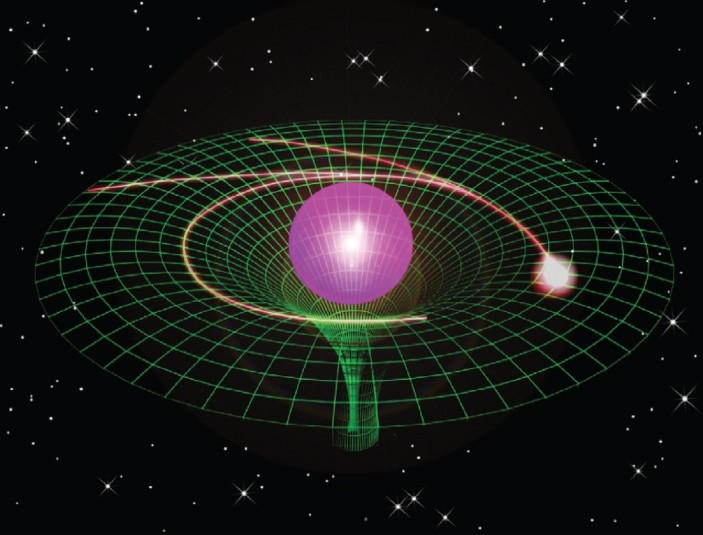
\includegraphics[height=3.5cm]{curvature}
            \vspace{-1ex}
            \caption*{\scriptsize \lbrack Cowen (2013)\rbrack}
            %! suppress = FigureNotReferenced
            \label{fig:figure}
        \end{figure}
    \end{frame}

    \begin{frame}{Gliederung}
        \tableofcontents[pausesections]
    \end{frame}


    \section{Konstruktive Gravitation}\label{sec:constructive-gravity}

    \begin{frame}{Space tells matter how to move \ldots}
        \begin{itemize}
            \item Punktmassen
            \[ S = m \int \sqrt{{\color{blue}g(}\dot\gamma(\lambda),\dot\gamma(\lambda){\color{blue})}} d\lambda \]
            \item Maxwell-Elektrodynamik
            \[ S = \int {\color{blue}\sqrt{-g}g^{ac}g^{bd}} F_{ab} F_{cd} d^4 x \]
            \item $\rightarrow$ Gesamtes Standardmodell ist metrisch
            \item Prädiktiv nur, wenn Dynamik der Raumzeitmetrik bekannt!
        \end{itemize}
    \end{frame}

    \begin{frame}{\ldots{} Matter tells space how to curve}
        \begin{itemize}
            \item Gravitation ist dynamische Theorie der Raumzeitmetrik!
            \item Allgemeine Relativitätstheorie {\scriptsize\lbrack Einstein (1915)\rbrack}
            \begin{gather*}
                S = \int \sqrt{-g} (R - 2 \Lambda) d^4 x \\
                G_{ab} = T_{ab}
            \end{gather*}
        \end{itemize}
    \end{frame}

    \begin{frame}{Eindeutigkeit der Allgemeinen Relativitätstheorie}
        Einsteins Allgemeine Relativitätstheorie (ART) ist die einzig mögliche dynamische Theorie
        der Raumzeitmetrik \pause
        \begin{itemize}
            \setlength{\belowdisplayskip}{-10pt}
            \item \textbf{Hochman, Kuchař, Teitelboim (1976):} \\ ART ist eindeutige Darstellung der Dirac-Algebra
            \begin{align*}
                \{ D(\vec N), D(\vec M) \} &= -D(\mathcal L_{\vec M} \vec N) \\
                \{ H(N), D(\vec M) \} &= -H(\mathcal L_{\vec M} N) \\
                \{ H(N), H(M) \} &= H(g^{\alpha\beta}(M\partial_\alpha N - N\partial_\alpha M))
            \end{align*} \pause
            \item \textbf{Lovelock (1969):} \\ Allgemeine Kovarianz $\Rightarrow$ Einstein-Gleichungen \pause
            \item \textbf{Deser (1970):} \\ Linearisierte ART + Selbstwechselwirkung $\Rightarrow$ ART
        \end{itemize}
    \end{frame}

    \begin{frame}{Konstruktive Gravitation}
        \begin{itemize}
            \item \textbf{Grundidee der Konstruktiven Gravitation:} \\
            Modifizierte Gravitation ergibt sich aus der Betrachtung neuartiger Materietheorien
            \item \textbf{Konstruktionsprinzip:} \\
            Reproduktion der Eindeutigkeitstheoreme für Maxwell-Einstein
            \item \textbf{Unterteilung}: \\
            Je nach Art des Eindeutigkeitstheorems
        \end{itemize}
    \end{frame}

    \begin{frame}{Kanonische Konstruktive Gravitation}
        \begin{itemize}
            \item HKT für beliebige tensorielle Geometrien
            \item Prinzip: Constraint-Algebra implementiert Dirac-Algebra
            \item $\Leftrightarrow$ unendliches System von PDEs für Lagrangedichte
            \item Lösungsstrategien: Perturbativ, Symmetriereduktion
        \end{itemize}

        \raggedleft\scriptsize \lbrack Giesel et al.\ (2012); Schuller, Witte (2014); Düll et al.\ (2019)\rbrack
    \end{frame}

    \begin{frame}{Kovariante Konstrutive Gravitation}
        \begin{itemize}
            \item Postulat der allgemeinen Kovarianz direkt für Lagrangian
            \item Verwandt mit Lovelock und Deser
            \item Manifest \emph{Kovariant}, da ohne 3+1-Split
            \item Zusätzliche Forderung nach kausaler Kompatibilität
        \end{itemize}

        \raggedleft\scriptsize \lbrack N.A., Reinhart (2020); N.A.\ (2020)\rbrack
    \end{frame}


    \section{Kovariante Implementierung}\label{sec:covariant-constructive-gravity}

    \begin{frame}{Lagrange-Formalismus}
        \begin{itemize}
            \item Differenzierbare Raumzeitmannigfaltigkeit $M$
            \item Geometrie ist Tensorbündel $E \xrightarrow{\pi} M$
            \begin{itemize}
                \item Metrisches Bündel $\operatorname{Sym}(T^0_2 M)$
                \item Bi-metrisches Bündel $\operatorname{Sym}(T^0_2 M) \oplus_M \operatorname{Sym}(T^0_2 M)$
                \item Area-metrisches Bündel als Sub-Bündel von $T^4_0 M$
            \end{itemize}
            \item Lagrangian $\mathscr L \in \bigwedge^n_0 \pi_2$ ist eine horizontale $n$-Form auf dem
            2.\ Jet-Bündel $J^2 E \xrightarrow{\pi_2} M$
            \item In Koordinaten
            \[ \mathscr{L} = \alert{L(x^i, u^A, u^A_i, u^A_{ij})} dx^1 \wedge \dots \wedge dx^n \]
        \end{itemize}
    \end{frame}

    \begin{frame}{Allgemeine Kovarianz}
        \begin{itemize}
            \item $\mathscr L$ invariant unter Diffeomorphismen $\varphi\in\operatorname{Diff}(M)$
            \[ \Leftrightarrow {\underbrace{j^2(\varphi_E)}_{\mathclap{\text{Lift auf 2.\ Jet-Bündel}}}}^\ast\mathscr{L} = \mathscr{L} \]
            \item In lokalen Koordinaten
            \[ L\circ j^2(\varphi_E) = \lvert d\varphi\rvert^{-1} L \]
            \item Infinitesimale Diffeo's
            \begin{align*}
                x^p &\mapsto x^p + \xi^p \\
                G^A &\mapsto G^A + \underbrace{\gmc{A}{B}{n}{m}}_{\mathclap{\text{Gotay-Marsden-Koeffizienten}}} G^B \xi^n_m
            \end{align*}
        \end{itemize}
    \end{frame}

    \begin{frame}{\"Aquivarianzgleichungen}
        \setlength{\belowdisplayskip}{-10pt}
        \begin{align*}
            0 =& {\color{blue}L_{,m}} \\
            0 =& {\color{blue}L_{:A}} {\color{mLightBrown}\gmc{A}{B}{n}{m}} {\color{purple}u^B} + {\color{blue}L_{:A}} \left\lbrack {\color{mLightBrown}\gmc{A}{B}{n}{m}} \delta^q_p - \delta^A_B \delta^q_m \delta^n_p \right\rbrack {\color{purple}u^B_q} \\
            & + {\color{blue}L_{:A}^{\hphantom{:A}I}} \left\lbrack {\color{mLightBrown}\gmc{A}{B}{n}{m}} \delta^J_I - 2\delta^A_B J^{pn}_I I^J_{pm}\right\rbrack {\color{purple}u^B_J} + {\color{blue}L} \delta^n_m \\
            0 =& {\color{blue}L_{:A}^{\hphantom{:A}(p\mid}} {\color{mLightBrown}\gmc{A}{B}{\mid n)}{m}} {\color{purple}u^B} + {\color{blue}L_{:A}^{\hphantom{:A}I}}\left\lbrack {\color{mLightBrown}\gmc{A}{B}{(n}{m}} 2 J^{p)q}_I - \delta^A_B J^{pn}_I \delta^q_m\right\rbrack {\color{purple}u^B_q} \\
            0 =& {\color{blue}L_{:A}^{\hphantom{:A}I}} {\color{mLightBrown}\gmc{A}{B}{(n}{m}} J^{pq)}_I {\color{purple}u^B}
        \end{align*}
        \begin{itemize}
            \item System aus 140 linearen PDEs erster Ordnung
            \item Geometrieabhängigkeit nur in {\color{mLightBrown}Gotay-Marsden-Koeff.}
            \item Lösungen des Systems sind Kandidaten für Gravitation!
        \end{itemize}
    \end{frame}

    \begin{frame}{Eigenschaften der Äquivarianzgleichungen}
        \begin{itemize}
            \item \textbf{Theorem:} Die Äquivarianzgleichungen sind
            \alert{involutiv} und folglich \alert{formal integrierbar}.
            \item Folgt aus der Involutionstheorie für PDEs {\scriptsize \lbrack Seiler\rbrack}
            \item Fundamentale Bedeutung für konstruktiven Ansatz
            \begin{itemize}
                \item Aussagen über den Lösungsraum \\ $\rightarrow$ exakte Lösung
                \item Formaler Potenzreihenansatz \\ $\rightarrow$ perturbative Lösung
            \end{itemize}
            \item Nicht ableitbar im kanonischen Bild!
        \end{itemize}
    \end{frame}

    \begin{frame}{Exakte Lösung: Einstein}
        \begin{itemize}
            \item Zweites metrisches Jet-Bündel hat Dimension 154
            \item Äquivarianzgleichungen haben Rang 140
            \item Involutivität $\Rightarrow$ allgemeine Lösung
            \[ L = \sqrt{-g} \cdot F(\psi_1,\ldots,\psi_{14}) \]
            mit beliebiger Funktion $F$ und 14 Krümmungsskalaren $\Psi_i$
            \item Beschränkung auf 2.\ Ableitungsordnung $\Rightarrow$ \alert{Einstein-Hilbert}
            \[ L = \frac{1}{2\kappa}\sqrt{-g}(\underbrace{R}_{\psi_1} - 2\Lambda)\]
        \end{itemize}
    \end{frame}

    \begin{frame}{Neuartige Materie}
        \textbf{Beispiel bi-metrische Theorie:}\\ Skalarfelder gekoppelt an zwei verschiedene Metriken
            {\setlength{\belowdisplayskip}{-5pt}
        \[ L = {\color{red}\sqrt{-g} g^{ab}} \phi_{,a}\phi_{,b} - m_\phi^2 \phi^2 + {\color{blue}\sqrt{-h} h^{ab}} \psi_{,a}\psi_{,b} - m_\psi^2 \psi^2 \]}
        \begin{itemize}
            \item Geometriebündel ist die Summe von zwei Metrikbündeln
            \item Gotay-Marsden-Koeffizienten $\Rightarrow$ Äquivarianzgleichungen
            \item Materie-Lichtkegel
            \[ P(k) = {\color{red}g}(k,k) {\color{blue}h}(k,k) = 0 \]
        \end{itemize}
    \end{frame}


    \section{Störungstheorie}\label{sec:stoerungstheorie}

    \begin{frame}{Potenzreihenansatz}
        \begin{itemize}
            \item Störungsansatz für Lagrangian
            \setlength{\belowdisplayskip}{-10pt}
            \begin{align*}
                G^A &= N^A + H^A \\
                L &= {\color{green}a} + {\color{blue}a_A H^A + a_A^{\hphantom Ai} H^A_{\hphantom{A},i} + a_A^{\hphantom AI} H^A_{\hphantom{A},I}} + {\color{violet}a_{AB} H^A H^B + {}} \ldots
            \end{align*}
            \item Iterative Lösung
            \begin{itemize}
                \item \makebox[11em]{Ansatz in PDE\hfill} $\Rightarrow$ {\color{blue}bestimmt $a_{\dots}$ zu 1.\ Ordnung}
                \item \makebox[11em]{Ansatz in 1.\ Prolongation\hfill} $\Rightarrow$ {\color{violet}bestimmt $a_{\dots}$ zu 2.\ Ordnung}
                \item etc.\ bis gewünschte Ordnung
                \item Garantiert durch \alert{Involutivität}!
            \end{itemize}
            \item Perturbative Kovariante Konstruktive Gravitation
            \begin{itemize}
                \item $n=0$: Minkowski-Hintergrund
                \item $n=2$: Linearisierte Gravitation
                \item $n=3$: Gravitative Selbstwechselwirkung
                \item \ldots
            \end{itemize}
        \end{itemize}
    \end{frame}

    \begin{frame}{Lorentzinvariante Ansätze}
        \begin{itemize}
            \item \textbf{Beobachtung:} \\ $SO(1,3)$-Invarianz von $N$ überträgt sich auf $a, a_A, \ldots$
            \item $\Rightarrow$ $a, a_A, \ldots$ zusammengesetzt aus ${\color{blue}\eta}$ und ${\color{blue}\epsilon}$
            \item Bsp.\ für metrische Theorien:
            \begin{itemize}
                \item $a_{ab} = A \cdot {\color{blue}\eta_{ab}}$
                \item $a_{ab}^{\hphantom{ab}i} = 0$
                \item $a_{abcd} = A\cdot {\color{blue}\eta_{ab} \eta_{cd}} + B\cdot {\color{blue}\eta_{ac} \eta_{bd}} + C\cdot {\color{blue}\eta_{ad} \eta_{bc}} + D \cdot {\color{blue}\epsilon_{abcd}}$
            \end{itemize}
            \item Haskell-Implementierung auf Workstation-Hardware: \\
            Erzeugung von Ansätzen mit bis zu 18 Raumzeitindizes
        \end{itemize}
    \end{frame}

    \begin{frame}{Perturbative Äquivarianzgleichungen}
        \begin{itemize}
            \item Für erzeugte Ansätze bleibt zu lösen (hier bis 2.\ Ordnung)
            \begin{align*}
                0 &{} = {\color{blue}a_A} \gmc{A}{B}{n}{m} N^B + {\color{blue}a} \delta^n_m \\
                0 &{} = {\color{blue}a_A^{\hphantom AI}}\gmc{A}{B}{(n}{m} J^{pq)}_I N^B
            \end{align*}
            \begin{align*}
                0 &{} = {\color{blue}a_A} \gmc{A}{B}{n}{m} + 2 {\color{blue}a_{AB}} \gmc{A}{C}{n}{m} N^C + {\color{blue}a_B} \delta^n_m \\
                0 &{} = {\color{blue}a_A^{\hphantom AI}}\lbrack \gmc{A}{B}{n}{m} \delta^J_I - 2\delta^A_B J^{pn}_I I^J_{pm}\rbrack + {\color{blue}a_{AB}^{\hphantom{AB}J}}\gmc{A}{C}{n}{m} N^C + {\color{blue}a_B^{\hphantom BJ}} \delta^n_m \\
                0 &{} = 2{\color{blue}a_{A \hphantom pB}^{\hphantom A(p\hphantom Bq\mid}} \gmc{A}{C}{\mid n)}{m} N^C + {\color{blue}a_A^{\hphantom AI}}\lbrack \gmc{A}{B}{(n}{m} 2J^{p)q}_I - \delta^A_B J^{pn}_I \delta^q_m\rbrack \\
                0 &{} = {\color{blue}a_{BA}^{\hphantom{BA}I}} \gmc{A}{C}{(n}{m} J^{pq)}_I N^C + {\color{blue}a_A^{\hphantom AI}}\gmc{A}{B}{(n}{m} J^{pq)}_I
            \end{align*}
            \item Lineares System mit rationalen Koeffizienten \\
            $\Rightarrow$ exakte Lösungen leicht mit Computer bestimmbar (fraction-free Gaussian elimination)
        \end{itemize}
    \end{frame}

    \begin{frame}[fragile]{Tensorkalkül mit dem Computer}
        \begin{itemize}
            \item Auswertung der Äquivarianzgleichungen nicht trivial
            \item $\Rightarrow$ Umsetzung in Haskell
            \begin{itemize}
                \item Abbildung des Tensorkalküls im Typsystem
                \item Typsichere DSL für Operationen (Produkte, Summen, \ldots)
                \item Definition von benötigten Basistensoren
                \item Auswerten und Lösen der linearen Systeme
            \end{itemize}
        \end{itemize}
        \begin{figure}
            \begin{minted}[fontsize=\tiny]{haskell}
diffeoEq1A :: (Num v, Eq v, MonadError String m) =>
              T v -> T v -> m (T v)
diffeoEq1A ansatz4 ansatz8 = do
    e1 <- fmap contractT $
          (.* c1) =<< relabelT (VSpace "STArea" 21) [("A","B")] ansatz4
    e2 <- (scalarT 2 .*) . contractT =<< ((ansatz8 .*) =<< (c2 .* n))
    e3 <- (scalarT (-1) .*) =<< (ansatz4 .* d)
    fmap removeZerosT $ (e3 .+) =<< (e1 .+ e2)
  where
    n  = someFlatAreaCon  "ST" "C"
    c1 = someInterAreaCon "ST" "m" "n" "B" "A"
    c2 = someInterAreaCon "ST" "m" "n" "B" "C"
    d  = someDelta        "ST" 4 "m" "n"
            \end{minted}
            %! suppress = FigureNotReferenced
            \label{fig:haskell}
        \end{figure}
    \end{frame}

    \begin{frame}{Perturbative Kausale Kompatibilit\"at}
        \begin{itemize}
            \item Expansion der beteiligten Polynome
            \[ P(k) = P^{(0)}(k) + P^{(1)}_A(k) H^A + P^{(2)}_{AB}(k) H^A H^B + \ldots \]
            \item $P^{(i)}_{\dots}$ ergeben sich aus Koeffizienten $a, a_A, \ldots$
            \item Perturbative Gleichsetzung der Kausalitäten
        \end{itemize}
    \end{frame}


    \section{Anwendung: Gravitationswellen von Doppelbrechender Materie}\label{sec:anwendung}

    \begin{frame}{Generalized Linear Electrodynamics}
        \begin{itemize}
            \item „premetric electrodynamics” {\scriptsize \lbrack Hehl, Obukhov (2003)\rbrack}
            \item Allg.\ lineare Relation für \textit{Anregungen} und \textit{Feldstärken}
            \[
                H^{ab} = \alert{G^{abcd}} F_{cd}
            \]
            \item Quartischer Lichtkegel \[ 0 = P(k) = -\frac{1}{24} \omega_G^2 \epsilon_{mnpq} \epsilon_{rstu} \alert{G^{mnra} G^{bpsc} G^{dqtu}} k_a k_b k_c k_d \]
            $\Rightarrow$ \textbf{Doppelbrechung im Vakuum!}
        \end{itemize}
    \end{frame}

    \begin{frame}{Area-Metrik}
        \begin{itemize}
            \item \alert{$G$} ist die \alert{Area-Metrik} mit Symmetrien
            \[ G^{\color{blue}ab\color{olive}cd} = -G^{\color{blue}ba\color{olive}cd} = G^{\color{olive}cd\color{blue}ab} \]
            \item Area-Metrik-Bündel $E_\text{Area}$ hat Faserdimension 21
            \item \alert{$G$} bestimmt GLED-Wirkung \[ S = \int \omega_{\alert{G}} \alert{G^{abcd}} F_{ab} F_{cd} d^4 x \]
            \item Maxwell: $G^{abcd} = g^{ac} g^{bd} - g^{ad} g^{bc}$ (+ Dichte)
        \end{itemize}
    \end{frame}

    \begin{frame}
        \textbf{Fragestellung:} \\
        Gegeben ein Doppelsternsystem aus doppelbrechender Materie, wie wirkt es
        gravitativ auf Testmaterie und auf sich selbst?

        \alert{
            \textbf{Antwort:} \\
            Konstruktion einer kompatiblen Gravitationstheorie!
        }
    \end{frame}

    \begin{frame}{Konstruktion der Area-Metrik-Gravitation}
        \begin{itemize}
            \item Intertwiner und Gotay-Marsden-Koeffizienten
            \begin{gather*}
                I \colon E_\text{Area} \rightarrow T^4_0 M \\
                J  \colon T^4_0 M \rightarrow E_\text{Area} \\
                \gmc{A}{B}{n}{m} = 4 I^{pqrn}_B J_{pqrm}^A
            \end{gather*}
            \item Äquivarianzgleichungen: \\
            140 PDE mit 319 unabhängigen Variablen
            \item Keine exakte Lösung mit nichttrivialer Dynamik bekannt!
        \end{itemize}
    \end{frame}

    \begin{frame}{Perturbative Konstruktion der Area-Metrik-Gravitation}
        \begin{itemize}
            \item Naheliegender Lorentz-Invarianter Ausgangspunkt
            \[
                N^{abcd} = \eta^{ac} \eta^{bd} - \eta^{ad} \eta^{bc} + \epsilon^{abcd}
            \]
            $\Rightarrow$ Reduziert GLED zu Maxwell auf Minkowski!
            \item Computergenerierte Ansätze bis zur 3.\ Ordnung
            \footnotesize
            \begin{table}
                \centering
                \begin{tabular}{l r r}
                    \toprule
                    Ansatz                                            & Dimension \\
                    \midrule
                    $a_A^{\hphantom AI}$                              & 3         \\ \addlinespace[2pt]
                    $a_{AB}$                                          & 6         \\ \addlinespace[2pt]
                    $a_{A\hphantom pB}^{\hphantom Ap\hphantom Bq}$    & 15        \\ \addlinespace[2pt]
                    $a_{AB}^{\hphantom{AB}I}$                         & 16        \\ \addlinespace[2pt]
                    $a_{ABC}$                                         & 15        \\ \addlinespace[2pt]
                    $a_{AB\hphantom pC}^{\hphantom{AB}p\hphantom Cq}$ & 110       \\ \addlinespace[2pt]
                    $a_{ABC}^{\hphantom{ABC}I}$                       & 72        \\ \addlinespace[2pt]
                    \bottomrule
                \end{tabular}\label{tab:ansaetze}
            \end{table}
        \end{itemize}
    \end{frame}

    \begin{frame}{Perturbative Konstruktion der Area-Metrik-Gravitation}
        \begin{itemize}
            \item Auswertung und Lösung der Äquivarianzgleichungen
            \begin{itemize}
                \item Lagrangian parametrisiert durch 50 Konstanten
                \item \alert{10 unabhängige Parameter für linearisierte Euler-Lagrange-Gleichungen} \\
                $\rightarrow$ Am meisten Relevanz für hier diskutierte Dynamik
            \end{itemize}
            \item Kausalität zu dieser Ordnung immer kompatibel mit GLED!
        \end{itemize}
    \end{frame}

    \begin{frame}{Raum-Zeit-Split}
        \begin{itemize}
            \item Blätterung der Raumzeit in räumliche Hyperflächen
            \item Induziert Aufteilung der 21 Freiheitsgrade $G^{abcd}$ \\ $\Rightarrow$ Lapse + Shift + Räumliche Tensoren
            \item Skalar-Vektor-Tensor-Zerlegung + Eichfixierung:
            \begin{itemize}
                \item \makebox[3.8cm]{3 TT-Tensoren\hfill} {\color{blue}$U^{\alpha\beta}$}, {\color{alert}$V^{\alpha\beta}$}, {\color{alert}$W^{\alpha\beta}$}
                \item \makebox[3.8cm]{3 Transversale Vektoren\hfill} {\color{blue}$B^\alpha$}, {\color{alert}$U^\alpha$}, {\color{alert}$W^\alpha$}
                \item \makebox[3.8cm]{5 Longitudinale Skalare\hfill} {\color{blue}$A$}, {\color{blue}$\tilde U$}, {\color{alert}$\tilde V$}, {\color{alert}$V$}, {\color{alert}$W$}
            \end{itemize}
        \end{itemize}
        \raggedleft
        {\color{blue}metrische Moden} \\
        $\color{blue}G_{\text{metrisch}}^{abcd} = g^{ac} g^{bd} - g^{ad} g^{bc}$ \\
        {\color{alert}nicht-metrische Moden}
    \end{frame}

    \begin{frame}{Linearisierte 3+1-Feldgleichungen}
        \begin{itemize}
            \item Beseitigung unphysikalischer Artefakte
            \begin{itemize}
                \item Divergierende Moden bei Wellengleichungen
                \item Fernfeld-Modifikationen der lin.\ Schwarzschild-Lösung
            \end{itemize}
            \item $\Rightarrow$ Reduktion von 10 auf 7 Konstanten
            \item Reduzierte Feldgleichungen ($X = W,V,U^\alpha,V^\alpha,V^{\alpha\beta},W^{\alpha\beta}$)
            \begin{gather*}
                \begin{aligned}
                    \color{blue}\text{(Quellterme)} &\color{blue}= \Box U^{\alpha\beta} \\
                    \color{red}\text{(Quellterme)} &\color{red}= \Box X + \nu^2 X \\
                    \color{red}\text{(Quellterme)} &\color{red}= \Box \tilde V + \mu^2 \tilde V \\
                \end{aligned} \\
                \color{blue}\text{Constraint-Gleichungen für }A, B^\alpha, \tilde U
            \end{gather*}
        \end{itemize}
    \end{frame}

    \begin{frame}[fragile]{Doppelsternsystem}
        \begin{center}
            \begin{tikzpicture}
                \fill[visible on=<1->] ({1.5*cos(45)},0,{1.5*sin(45)}) circle (0.14) node[anchor=north west,outer sep=1pt]{$m_1$};
                \fill[visible on=<1->] ({-3.5*cos(45)},0,{-3.5*sin(45)}) circle (0.14) node[anchor=north west,outer sep=1pt]{$m_2$};

                \begin{scope}[canvas is zx plane at y=0]
                    \draw[visible on=<2->,decoration={markings, mark=at position 0.3 with {\arrow[scale=1.5]{Latex}}},postaction={decorate}] (0,0) circle (1.5);
                    \draw[visible on=<2->,decoration={markings, mark=at position 0.8 with {\arrow[scale=1.5]{Latex}}},postaction={decorate}] (0,0) circle (3.5);
                \end{scope}

                \draw[visible on=<3->,decoration={snake,segment length=6pt,post length=6pt},decorate,-{Latex}] (2.4,-0.9,-0.5) -- (4,-1.5,-0.5);
                \draw[visible on=<3->,decoration={snake,segment length=6pt,post length=6pt},decorate,-{Latex}] (2.4,-0.9,0) -- (4,-1.5,0);
                \draw[visible on=<3->,decoration={snake,segment length=6pt,post length=6pt},decorate,-{Latex}] (2.4,-0.9,0.5) -- (4,-1.5,0.5);

                \draw[visible on=<3->] (5.3,-1.6,0) node{\pgfuseimage{ligo}};
                \draw[visible on=<3->] (5.3,-2.25,0) node{\tiny\lbrack Abbott et al.\ (2016)\rbrack};
            \end{tikzpicture}
        \end{center}

        \vspace{-2em}
        Iterative Lösung: \scriptsize \lbrack vgl.\ Poisson, Will (2014)\rbrack \footnotesize
        \begin{enumerate}
            \item<2-> Trajektorien zu 1.\ Ordnung \\
            $\Rightarrow$ Kreisförmige Orbits mit \alert{modifiziertem Kepler-Gesetz}
            \[\omega^2 = \frac{Gm}{r^3}\lbrack 1 + \alert{\underbrace{f(r)}_{\mathclap{\beta(1+\mu r)\mathrm e^{-\mu r}}}} \rbrack \] \pause
            \vspace{-1em}
            \item<3-> Wellengleichung für 2.\ Ordnung mit Quelltermen aus 1.\ Ordnung\\
            $\Rightarrow$ \alert{Strahlung auf $U^{\alpha\beta}$-Mode mit $f(r)$ korrigiert} \\
            $\Rightarrow$ \alert{Moden mit Masse $\nu$ strahlen ab $2\omega > \nu$}
        \end{enumerate}
    \end{frame}

    \begin{frame}{Strahlungsverluste}
        \begin{itemize}
            \item Aus Diffeo-Invarianz folgt zweites Noether-Theorem
            \[ -D_n \lbrack\frac{\delta L}{\delta G^A} \gmc{A}{B}{n}{m} G^B\rbrack = \frac{\delta L}{\delta G^A} G^A_{,m} \]
            \item Angewandt auf Doppelsternsystem in masseloser Strahlungsphase:
            \[ \left(\frac{1 + \alert{f(r)}}{r}\right)^{\scalebox{1.5}{\cdot}} = \frac{64}{5} \eta c \frac{1}{r^2} \left(\frac{Gm}{c^2 r}\lbrack 1+\alert{f(r)}\rbrack\right)^3\]
            \alert{Korrektur der metrischen ODE mit $f(r)$!}
        \end{itemize}
    \end{frame}

    \begin{frame}{Strahlungsverluste}
        \begin{figure}
            \centering
            \begin{subfigure}{.49\textwidth}
                \centering
                \resizebox{1.1\textwidth}{!}{%% Creator: Matplotlib, PGF backend
%%
%% To include the figure in your LaTeX document, write
%%   \input{<filename>.pgf}
%%
%% Make sure the required packages are loaded in your preamble
%%   \usepackage{pgf}
%%
%% Figures using additional raster images can only be included by \input if
%% they are in the same directory as the main LaTeX file. For loading figures
%% from other directories you can use the `import` package
%%   \usepackage{import}
%%
%% and then include the figures with
%%   \import{<path to file>}{<filename>.pgf}
%%
%% Matplotlib used the following preamble
%%   \usepackage{fontspec}
%%
\begingroup%
\makeatletter%
\begin{pgfpicture}%
\pgfpathrectangle{\pgfpointorigin}{\pgfqpoint{5.546080in}{3.427666in}}%
\pgfusepath{use as bounding box, clip}%
\begin{pgfscope}%
\pgfsetbuttcap%
\pgfsetmiterjoin%
\definecolor{currentfill}{rgb}{1.000000,1.000000,1.000000}%
\pgfsetfillcolor{currentfill}%
\pgfsetlinewidth{0.000000pt}%
\definecolor{currentstroke}{rgb}{1.000000,1.000000,1.000000}%
\pgfsetstrokecolor{currentstroke}%
\pgfsetdash{}{0pt}%
\pgfpathmoveto{\pgfqpoint{0.000000in}{0.000000in}}%
\pgfpathlineto{\pgfqpoint{5.546080in}{0.000000in}}%
\pgfpathlineto{\pgfqpoint{5.546080in}{3.427666in}}%
\pgfpathlineto{\pgfqpoint{0.000000in}{3.427666in}}%
\pgfpathclose%
\pgfusepath{fill}%
\end{pgfscope}%
\begin{pgfscope}%
\pgfsetbuttcap%
\pgfsetmiterjoin%
\definecolor{currentfill}{rgb}{1.000000,1.000000,1.000000}%
\pgfsetfillcolor{currentfill}%
\pgfsetlinewidth{0.000000pt}%
\definecolor{currentstroke}{rgb}{0.000000,0.000000,0.000000}%
\pgfsetstrokecolor{currentstroke}%
\pgfsetstrokeopacity{0.000000}%
\pgfsetdash{}{0pt}%
\pgfpathmoveto{\pgfqpoint{0.693260in}{0.377043in}}%
\pgfpathlineto{\pgfqpoint{4.991472in}{0.377043in}}%
\pgfpathlineto{\pgfqpoint{4.991472in}{3.016346in}}%
\pgfpathlineto{\pgfqpoint{0.693260in}{3.016346in}}%
\pgfpathclose%
\pgfusepath{fill}%
\end{pgfscope}%
\begin{pgfscope}%
\pgfsetbuttcap%
\pgfsetroundjoin%
\definecolor{currentfill}{rgb}{0.000000,0.000000,0.000000}%
\pgfsetfillcolor{currentfill}%
\pgfsetlinewidth{0.803000pt}%
\definecolor{currentstroke}{rgb}{0.000000,0.000000,0.000000}%
\pgfsetstrokecolor{currentstroke}%
\pgfsetdash{}{0pt}%
\pgfsys@defobject{currentmarker}{\pgfqpoint{0.000000in}{-0.048611in}}{\pgfqpoint{0.000000in}{0.000000in}}{%
\pgfpathmoveto{\pgfqpoint{0.000000in}{0.000000in}}%
\pgfpathlineto{\pgfqpoint{0.000000in}{-0.048611in}}%
\pgfusepath{stroke,fill}%
}%
\begin{pgfscope}%
\pgfsys@transformshift{0.888633in}{0.377043in}%
\pgfsys@useobject{currentmarker}{}%
\end{pgfscope}%
\end{pgfscope}%
\begin{pgfscope}%
\definecolor{textcolor}{rgb}{0.000000,0.000000,0.000000}%
\pgfsetstrokecolor{textcolor}%
\pgfsetfillcolor{textcolor}%
\pgftext[x=0.888633in,y=0.279821in,,top]{\color{textcolor}\rmfamily\fontsize{10.000000}{12.000000}\selectfont \(\displaystyle {0}\)}%
\end{pgfscope}%
\begin{pgfscope}%
\pgfsetbuttcap%
\pgfsetroundjoin%
\definecolor{currentfill}{rgb}{0.000000,0.000000,0.000000}%
\pgfsetfillcolor{currentfill}%
\pgfsetlinewidth{0.803000pt}%
\definecolor{currentstroke}{rgb}{0.000000,0.000000,0.000000}%
\pgfsetstrokecolor{currentstroke}%
\pgfsetdash{}{0pt}%
\pgfsys@defobject{currentmarker}{\pgfqpoint{0.000000in}{-0.048611in}}{\pgfqpoint{0.000000in}{0.000000in}}{%
\pgfpathmoveto{\pgfqpoint{0.000000in}{0.000000in}}%
\pgfpathlineto{\pgfqpoint{0.000000in}{-0.048611in}}%
\pgfusepath{stroke,fill}%
}%
\begin{pgfscope}%
\pgfsys@transformshift{1.446843in}{0.377043in}%
\pgfsys@useobject{currentmarker}{}%
\end{pgfscope}%
\end{pgfscope}%
\begin{pgfscope}%
\definecolor{textcolor}{rgb}{0.000000,0.000000,0.000000}%
\pgfsetstrokecolor{textcolor}%
\pgfsetfillcolor{textcolor}%
\pgftext[x=1.446843in,y=0.279821in,,top]{\color{textcolor}\rmfamily\fontsize{10.000000}{12.000000}\selectfont \(\displaystyle {2}\)}%
\end{pgfscope}%
\begin{pgfscope}%
\pgfsetbuttcap%
\pgfsetroundjoin%
\definecolor{currentfill}{rgb}{0.000000,0.000000,0.000000}%
\pgfsetfillcolor{currentfill}%
\pgfsetlinewidth{0.803000pt}%
\definecolor{currentstroke}{rgb}{0.000000,0.000000,0.000000}%
\pgfsetstrokecolor{currentstroke}%
\pgfsetdash{}{0pt}%
\pgfsys@defobject{currentmarker}{\pgfqpoint{0.000000in}{-0.048611in}}{\pgfqpoint{0.000000in}{0.000000in}}{%
\pgfpathmoveto{\pgfqpoint{0.000000in}{0.000000in}}%
\pgfpathlineto{\pgfqpoint{0.000000in}{-0.048611in}}%
\pgfusepath{stroke,fill}%
}%
\begin{pgfscope}%
\pgfsys@transformshift{2.005052in}{0.377043in}%
\pgfsys@useobject{currentmarker}{}%
\end{pgfscope}%
\end{pgfscope}%
\begin{pgfscope}%
\definecolor{textcolor}{rgb}{0.000000,0.000000,0.000000}%
\pgfsetstrokecolor{textcolor}%
\pgfsetfillcolor{textcolor}%
\pgftext[x=2.005052in,y=0.279821in,,top]{\color{textcolor}\rmfamily\fontsize{10.000000}{12.000000}\selectfont \(\displaystyle {4}\)}%
\end{pgfscope}%
\begin{pgfscope}%
\pgfsetbuttcap%
\pgfsetroundjoin%
\definecolor{currentfill}{rgb}{0.000000,0.000000,0.000000}%
\pgfsetfillcolor{currentfill}%
\pgfsetlinewidth{0.803000pt}%
\definecolor{currentstroke}{rgb}{0.000000,0.000000,0.000000}%
\pgfsetstrokecolor{currentstroke}%
\pgfsetdash{}{0pt}%
\pgfsys@defobject{currentmarker}{\pgfqpoint{0.000000in}{-0.048611in}}{\pgfqpoint{0.000000in}{0.000000in}}{%
\pgfpathmoveto{\pgfqpoint{0.000000in}{0.000000in}}%
\pgfpathlineto{\pgfqpoint{0.000000in}{-0.048611in}}%
\pgfusepath{stroke,fill}%
}%
\begin{pgfscope}%
\pgfsys@transformshift{2.563261in}{0.377043in}%
\pgfsys@useobject{currentmarker}{}%
\end{pgfscope}%
\end{pgfscope}%
\begin{pgfscope}%
\definecolor{textcolor}{rgb}{0.000000,0.000000,0.000000}%
\pgfsetstrokecolor{textcolor}%
\pgfsetfillcolor{textcolor}%
\pgftext[x=2.563261in,y=0.279821in,,top]{\color{textcolor}\rmfamily\fontsize{10.000000}{12.000000}\selectfont \(\displaystyle {6}\)}%
\end{pgfscope}%
\begin{pgfscope}%
\pgfsetbuttcap%
\pgfsetroundjoin%
\definecolor{currentfill}{rgb}{0.000000,0.000000,0.000000}%
\pgfsetfillcolor{currentfill}%
\pgfsetlinewidth{0.803000pt}%
\definecolor{currentstroke}{rgb}{0.000000,0.000000,0.000000}%
\pgfsetstrokecolor{currentstroke}%
\pgfsetdash{}{0pt}%
\pgfsys@defobject{currentmarker}{\pgfqpoint{0.000000in}{-0.048611in}}{\pgfqpoint{0.000000in}{0.000000in}}{%
\pgfpathmoveto{\pgfqpoint{0.000000in}{0.000000in}}%
\pgfpathlineto{\pgfqpoint{0.000000in}{-0.048611in}}%
\pgfusepath{stroke,fill}%
}%
\begin{pgfscope}%
\pgfsys@transformshift{3.121471in}{0.377043in}%
\pgfsys@useobject{currentmarker}{}%
\end{pgfscope}%
\end{pgfscope}%
\begin{pgfscope}%
\definecolor{textcolor}{rgb}{0.000000,0.000000,0.000000}%
\pgfsetstrokecolor{textcolor}%
\pgfsetfillcolor{textcolor}%
\pgftext[x=3.121471in,y=0.279821in,,top]{\color{textcolor}\rmfamily\fontsize{10.000000}{12.000000}\selectfont \(\displaystyle {8}\)}%
\end{pgfscope}%
\begin{pgfscope}%
\pgfsetbuttcap%
\pgfsetroundjoin%
\definecolor{currentfill}{rgb}{0.000000,0.000000,0.000000}%
\pgfsetfillcolor{currentfill}%
\pgfsetlinewidth{0.803000pt}%
\definecolor{currentstroke}{rgb}{0.000000,0.000000,0.000000}%
\pgfsetstrokecolor{currentstroke}%
\pgfsetdash{}{0pt}%
\pgfsys@defobject{currentmarker}{\pgfqpoint{0.000000in}{-0.048611in}}{\pgfqpoint{0.000000in}{0.000000in}}{%
\pgfpathmoveto{\pgfqpoint{0.000000in}{0.000000in}}%
\pgfpathlineto{\pgfqpoint{0.000000in}{-0.048611in}}%
\pgfusepath{stroke,fill}%
}%
\begin{pgfscope}%
\pgfsys@transformshift{3.679680in}{0.377043in}%
\pgfsys@useobject{currentmarker}{}%
\end{pgfscope}%
\end{pgfscope}%
\begin{pgfscope}%
\definecolor{textcolor}{rgb}{0.000000,0.000000,0.000000}%
\pgfsetstrokecolor{textcolor}%
\pgfsetfillcolor{textcolor}%
\pgftext[x=3.679680in,y=0.279821in,,top]{\color{textcolor}\rmfamily\fontsize{10.000000}{12.000000}\selectfont \(\displaystyle {10}\)}%
\end{pgfscope}%
\begin{pgfscope}%
\pgfsetbuttcap%
\pgfsetroundjoin%
\definecolor{currentfill}{rgb}{0.000000,0.000000,0.000000}%
\pgfsetfillcolor{currentfill}%
\pgfsetlinewidth{0.803000pt}%
\definecolor{currentstroke}{rgb}{0.000000,0.000000,0.000000}%
\pgfsetstrokecolor{currentstroke}%
\pgfsetdash{}{0pt}%
\pgfsys@defobject{currentmarker}{\pgfqpoint{0.000000in}{-0.048611in}}{\pgfqpoint{0.000000in}{0.000000in}}{%
\pgfpathmoveto{\pgfqpoint{0.000000in}{0.000000in}}%
\pgfpathlineto{\pgfqpoint{0.000000in}{-0.048611in}}%
\pgfusepath{stroke,fill}%
}%
\begin{pgfscope}%
\pgfsys@transformshift{4.237889in}{0.377043in}%
\pgfsys@useobject{currentmarker}{}%
\end{pgfscope}%
\end{pgfscope}%
\begin{pgfscope}%
\definecolor{textcolor}{rgb}{0.000000,0.000000,0.000000}%
\pgfsetstrokecolor{textcolor}%
\pgfsetfillcolor{textcolor}%
\pgftext[x=4.237889in,y=0.279821in,,top]{\color{textcolor}\rmfamily\fontsize{10.000000}{12.000000}\selectfont \(\displaystyle {12}\)}%
\end{pgfscope}%
\begin{pgfscope}%
\pgfsetbuttcap%
\pgfsetroundjoin%
\definecolor{currentfill}{rgb}{0.000000,0.000000,0.000000}%
\pgfsetfillcolor{currentfill}%
\pgfsetlinewidth{0.803000pt}%
\definecolor{currentstroke}{rgb}{0.000000,0.000000,0.000000}%
\pgfsetstrokecolor{currentstroke}%
\pgfsetdash{}{0pt}%
\pgfsys@defobject{currentmarker}{\pgfqpoint{0.000000in}{-0.048611in}}{\pgfqpoint{0.000000in}{0.000000in}}{%
\pgfpathmoveto{\pgfqpoint{0.000000in}{0.000000in}}%
\pgfpathlineto{\pgfqpoint{0.000000in}{-0.048611in}}%
\pgfusepath{stroke,fill}%
}%
\begin{pgfscope}%
\pgfsys@transformshift{4.796099in}{0.377043in}%
\pgfsys@useobject{currentmarker}{}%
\end{pgfscope}%
\end{pgfscope}%
\begin{pgfscope}%
\definecolor{textcolor}{rgb}{0.000000,0.000000,0.000000}%
\pgfsetstrokecolor{textcolor}%
\pgfsetfillcolor{textcolor}%
\pgftext[x=4.796099in,y=0.279821in,,top]{\color{textcolor}\rmfamily\fontsize{10.000000}{12.000000}\selectfont \(\displaystyle {14}\)}%
\end{pgfscope}%
\begin{pgfscope}%
\definecolor{textcolor}{rgb}{0.000000,0.000000,0.000000}%
\pgfsetstrokecolor{textcolor}%
\pgfsetfillcolor{textcolor}%
\pgftext[x=2.842366in,y=0.100932in,,top]{\color{textcolor}\rmfamily\fontsize{10.000000}{12.000000}\selectfont coordinate time \(\displaystyle t\)}%
\end{pgfscope}%
\begin{pgfscope}%
\pgfsetbuttcap%
\pgfsetroundjoin%
\definecolor{currentfill}{rgb}{0.000000,0.000000,0.000000}%
\pgfsetfillcolor{currentfill}%
\pgfsetlinewidth{0.803000pt}%
\definecolor{currentstroke}{rgb}{0.000000,0.000000,0.000000}%
\pgfsetstrokecolor{currentstroke}%
\pgfsetdash{}{0pt}%
\pgfsys@defobject{currentmarker}{\pgfqpoint{-0.048611in}{0.000000in}}{\pgfqpoint{-0.000000in}{0.000000in}}{%
\pgfpathmoveto{\pgfqpoint{-0.000000in}{0.000000in}}%
\pgfpathlineto{\pgfqpoint{-0.048611in}{0.000000in}}%
\pgfusepath{stroke,fill}%
}%
\begin{pgfscope}%
\pgfsys@transformshift{0.693260in}{0.651560in}%
\pgfsys@useobject{currentmarker}{}%
\end{pgfscope}%
\end{pgfscope}%
\begin{pgfscope}%
\definecolor{textcolor}{rgb}{0.000000,0.000000,0.000000}%
\pgfsetstrokecolor{textcolor}%
\pgfsetfillcolor{textcolor}%
\pgftext[x=0.418568in, y=0.603365in, left, base]{\color{textcolor}\rmfamily\fontsize{10.000000}{12.000000}\selectfont \(\displaystyle {0.5}\)}%
\end{pgfscope}%
\begin{pgfscope}%
\pgfsetbuttcap%
\pgfsetroundjoin%
\definecolor{currentfill}{rgb}{0.000000,0.000000,0.000000}%
\pgfsetfillcolor{currentfill}%
\pgfsetlinewidth{0.803000pt}%
\definecolor{currentstroke}{rgb}{0.000000,0.000000,0.000000}%
\pgfsetstrokecolor{currentstroke}%
\pgfsetdash{}{0pt}%
\pgfsys@defobject{currentmarker}{\pgfqpoint{-0.048611in}{0.000000in}}{\pgfqpoint{-0.000000in}{0.000000in}}{%
\pgfpathmoveto{\pgfqpoint{-0.000000in}{0.000000in}}%
\pgfpathlineto{\pgfqpoint{-0.048611in}{0.000000in}}%
\pgfusepath{stroke,fill}%
}%
\begin{pgfscope}%
\pgfsys@transformshift{0.693260in}{1.100523in}%
\pgfsys@useobject{currentmarker}{}%
\end{pgfscope}%
\end{pgfscope}%
\begin{pgfscope}%
\definecolor{textcolor}{rgb}{0.000000,0.000000,0.000000}%
\pgfsetstrokecolor{textcolor}%
\pgfsetfillcolor{textcolor}%
\pgftext[x=0.418568in, y=1.052329in, left, base]{\color{textcolor}\rmfamily\fontsize{10.000000}{12.000000}\selectfont \(\displaystyle {0.6}\)}%
\end{pgfscope}%
\begin{pgfscope}%
\pgfsetbuttcap%
\pgfsetroundjoin%
\definecolor{currentfill}{rgb}{0.000000,0.000000,0.000000}%
\pgfsetfillcolor{currentfill}%
\pgfsetlinewidth{0.803000pt}%
\definecolor{currentstroke}{rgb}{0.000000,0.000000,0.000000}%
\pgfsetstrokecolor{currentstroke}%
\pgfsetdash{}{0pt}%
\pgfsys@defobject{currentmarker}{\pgfqpoint{-0.048611in}{0.000000in}}{\pgfqpoint{-0.000000in}{0.000000in}}{%
\pgfpathmoveto{\pgfqpoint{-0.000000in}{0.000000in}}%
\pgfpathlineto{\pgfqpoint{-0.048611in}{0.000000in}}%
\pgfusepath{stroke,fill}%
}%
\begin{pgfscope}%
\pgfsys@transformshift{0.693260in}{1.549487in}%
\pgfsys@useobject{currentmarker}{}%
\end{pgfscope}%
\end{pgfscope}%
\begin{pgfscope}%
\definecolor{textcolor}{rgb}{0.000000,0.000000,0.000000}%
\pgfsetstrokecolor{textcolor}%
\pgfsetfillcolor{textcolor}%
\pgftext[x=0.418568in, y=1.501292in, left, base]{\color{textcolor}\rmfamily\fontsize{10.000000}{12.000000}\selectfont \(\displaystyle {0.7}\)}%
\end{pgfscope}%
\begin{pgfscope}%
\pgfsetbuttcap%
\pgfsetroundjoin%
\definecolor{currentfill}{rgb}{0.000000,0.000000,0.000000}%
\pgfsetfillcolor{currentfill}%
\pgfsetlinewidth{0.803000pt}%
\definecolor{currentstroke}{rgb}{0.000000,0.000000,0.000000}%
\pgfsetstrokecolor{currentstroke}%
\pgfsetdash{}{0pt}%
\pgfsys@defobject{currentmarker}{\pgfqpoint{-0.048611in}{0.000000in}}{\pgfqpoint{-0.000000in}{0.000000in}}{%
\pgfpathmoveto{\pgfqpoint{-0.000000in}{0.000000in}}%
\pgfpathlineto{\pgfqpoint{-0.048611in}{0.000000in}}%
\pgfusepath{stroke,fill}%
}%
\begin{pgfscope}%
\pgfsys@transformshift{0.693260in}{1.998450in}%
\pgfsys@useobject{currentmarker}{}%
\end{pgfscope}%
\end{pgfscope}%
\begin{pgfscope}%
\definecolor{textcolor}{rgb}{0.000000,0.000000,0.000000}%
\pgfsetstrokecolor{textcolor}%
\pgfsetfillcolor{textcolor}%
\pgftext[x=0.418568in, y=1.950256in, left, base]{\color{textcolor}\rmfamily\fontsize{10.000000}{12.000000}\selectfont \(\displaystyle {0.8}\)}%
\end{pgfscope}%
\begin{pgfscope}%
\pgfsetbuttcap%
\pgfsetroundjoin%
\definecolor{currentfill}{rgb}{0.000000,0.000000,0.000000}%
\pgfsetfillcolor{currentfill}%
\pgfsetlinewidth{0.803000pt}%
\definecolor{currentstroke}{rgb}{0.000000,0.000000,0.000000}%
\pgfsetstrokecolor{currentstroke}%
\pgfsetdash{}{0pt}%
\pgfsys@defobject{currentmarker}{\pgfqpoint{-0.048611in}{0.000000in}}{\pgfqpoint{-0.000000in}{0.000000in}}{%
\pgfpathmoveto{\pgfqpoint{-0.000000in}{0.000000in}}%
\pgfpathlineto{\pgfqpoint{-0.048611in}{0.000000in}}%
\pgfusepath{stroke,fill}%
}%
\begin{pgfscope}%
\pgfsys@transformshift{0.693260in}{2.447414in}%
\pgfsys@useobject{currentmarker}{}%
\end{pgfscope}%
\end{pgfscope}%
\begin{pgfscope}%
\definecolor{textcolor}{rgb}{0.000000,0.000000,0.000000}%
\pgfsetstrokecolor{textcolor}%
\pgfsetfillcolor{textcolor}%
\pgftext[x=0.418568in, y=2.399220in, left, base]{\color{textcolor}\rmfamily\fontsize{10.000000}{12.000000}\selectfont \(\displaystyle {0.9}\)}%
\end{pgfscope}%
\begin{pgfscope}%
\pgfsetbuttcap%
\pgfsetroundjoin%
\definecolor{currentfill}{rgb}{0.000000,0.000000,0.000000}%
\pgfsetfillcolor{currentfill}%
\pgfsetlinewidth{0.803000pt}%
\definecolor{currentstroke}{rgb}{0.000000,0.000000,0.000000}%
\pgfsetstrokecolor{currentstroke}%
\pgfsetdash{}{0pt}%
\pgfsys@defobject{currentmarker}{\pgfqpoint{-0.048611in}{0.000000in}}{\pgfqpoint{-0.000000in}{0.000000in}}{%
\pgfpathmoveto{\pgfqpoint{-0.000000in}{0.000000in}}%
\pgfpathlineto{\pgfqpoint{-0.048611in}{0.000000in}}%
\pgfusepath{stroke,fill}%
}%
\begin{pgfscope}%
\pgfsys@transformshift{0.693260in}{2.896378in}%
\pgfsys@useobject{currentmarker}{}%
\end{pgfscope}%
\end{pgfscope}%
\begin{pgfscope}%
\definecolor{textcolor}{rgb}{0.000000,0.000000,0.000000}%
\pgfsetstrokecolor{textcolor}%
\pgfsetfillcolor{textcolor}%
\pgftext[x=0.418568in, y=2.848183in, left, base]{\color{textcolor}\rmfamily\fontsize{10.000000}{12.000000}\selectfont \(\displaystyle {1.0}\)}%
\end{pgfscope}%
\begin{pgfscope}%
\definecolor{textcolor}{rgb}{0.000000,0.000000,0.000000}%
\pgfsetstrokecolor{textcolor}%
\pgfsetfillcolor{textcolor}%
\pgftext[x=0.363012in,y=1.696695in,,bottom,rotate=90.000000]{\color{textcolor}\rmfamily\fontsize{10.000000}{12.000000}\selectfont orbital period \(\displaystyle P / P_0\)}%
\end{pgfscope}%
\begin{pgfscope}%
\pgfpathrectangle{\pgfqpoint{0.693260in}{0.377043in}}{\pgfqpoint{4.298212in}{2.639303in}}%
\pgfusepath{clip}%
\pgfsetrectcap%
\pgfsetroundjoin%
\pgfsetlinewidth{1.505625pt}%
\definecolor{currentstroke}{rgb}{0.121569,0.466667,0.705882}%
\pgfsetstrokecolor{currentstroke}%
\pgfsetdash{}{0pt}%
\pgfpathmoveto{\pgfqpoint{0.888633in}{2.896378in}}%
\pgfpathlineto{\pgfqpoint{1.100029in}{2.816284in}}%
\pgfpathlineto{\pgfqpoint{1.303688in}{2.736758in}}%
\pgfpathlineto{\pgfqpoint{1.499845in}{2.657789in}}%
\pgfpathlineto{\pgfqpoint{1.688695in}{2.579380in}}%
\pgfpathlineto{\pgfqpoint{1.870472in}{2.501515in}}%
\pgfpathlineto{\pgfqpoint{2.045372in}{2.424192in}}%
\pgfpathlineto{\pgfqpoint{2.213629in}{2.347389in}}%
\pgfpathlineto{\pgfqpoint{2.375400in}{2.271118in}}%
\pgfpathlineto{\pgfqpoint{2.530879in}{2.195369in}}%
\pgfpathlineto{\pgfqpoint{2.680302in}{2.120113in}}%
\pgfpathlineto{\pgfqpoint{2.823825in}{2.045354in}}%
\pgfpathlineto{\pgfqpoint{2.961603in}{1.971095in}}%
\pgfpathlineto{\pgfqpoint{3.093872in}{1.897295in}}%
\pgfpathlineto{\pgfqpoint{3.220749in}{1.823973in}}%
\pgfpathlineto{\pgfqpoint{3.342429in}{1.751102in}}%
\pgfpathlineto{\pgfqpoint{3.459107in}{1.678650in}}%
\pgfpathlineto{\pgfqpoint{3.570901in}{1.606629in}}%
\pgfpathlineto{\pgfqpoint{3.677966in}{1.535025in}}%
\pgfpathlineto{\pgfqpoint{3.780499in}{1.463794in}}%
\pgfpathlineto{\pgfqpoint{3.878617in}{1.392937in}}%
\pgfpathlineto{\pgfqpoint{3.972475in}{1.322430in}}%
\pgfpathlineto{\pgfqpoint{4.062191in}{1.252269in}}%
\pgfpathlineto{\pgfqpoint{4.147922in}{1.182418in}}%
\pgfpathlineto{\pgfqpoint{4.229823in}{1.112835in}}%
\pgfpathlineto{\pgfqpoint{4.308012in}{1.043503in}}%
\pgfpathlineto{\pgfqpoint{4.382567in}{0.974437in}}%
\pgfpathlineto{\pgfqpoint{4.453645in}{0.905578in}}%
\pgfpathlineto{\pgfqpoint{4.521362in}{0.836895in}}%
\pgfpathlineto{\pgfqpoint{4.585836in}{0.768351in}}%
\pgfpathlineto{\pgfqpoint{4.647184in}{0.699901in}}%
\pgfpathlineto{\pgfqpoint{4.705484in}{0.631535in}}%
\pgfpathlineto{\pgfqpoint{4.760853in}{0.563194in}}%
\pgfpathlineto{\pgfqpoint{4.796099in}{0.517739in}}%
\pgfpathlineto{\pgfqpoint{4.796099in}{0.517739in}}%
\pgfusepath{stroke}%
\end{pgfscope}%
\begin{pgfscope}%
\pgfpathrectangle{\pgfqpoint{0.693260in}{0.377043in}}{\pgfqpoint{4.298212in}{2.639303in}}%
\pgfusepath{clip}%
\pgfsetbuttcap%
\pgfsetroundjoin%
\pgfsetlinewidth{1.505625pt}%
\definecolor{currentstroke}{rgb}{1.000000,0.498039,0.054902}%
\pgfsetstrokecolor{currentstroke}%
\pgfsetdash{{5.550000pt}{2.400000pt}}{0.000000pt}%
\pgfpathmoveto{\pgfqpoint{0.888633in}{2.896378in}}%
\pgfpathlineto{\pgfqpoint{1.104835in}{2.816699in}}%
\pgfpathlineto{\pgfqpoint{1.313066in}{2.737603in}}%
\pgfpathlineto{\pgfqpoint{1.513443in}{2.659127in}}%
\pgfpathlineto{\pgfqpoint{1.692759in}{2.586610in}}%
\pgfpathlineto{\pgfqpoint{1.852849in}{2.519312in}}%
\pgfpathlineto{\pgfqpoint{2.027163in}{2.443591in}}%
\pgfpathlineto{\pgfqpoint{2.212261in}{2.360746in}}%
\pgfpathlineto{\pgfqpoint{2.400134in}{2.274230in}}%
\pgfpathlineto{\pgfqpoint{2.581560in}{2.188261in}}%
\pgfpathlineto{\pgfqpoint{2.750833in}{2.105623in}}%
\pgfpathlineto{\pgfqpoint{2.906703in}{2.027087in}}%
\pgfpathlineto{\pgfqpoint{3.050265in}{1.952294in}}%
\pgfpathlineto{\pgfqpoint{3.183276in}{1.880517in}}%
\pgfpathlineto{\pgfqpoint{3.307457in}{1.811004in}}%
\pgfpathlineto{\pgfqpoint{3.424330in}{1.743054in}}%
\pgfpathlineto{\pgfqpoint{3.535069in}{1.676116in}}%
\pgfpathlineto{\pgfqpoint{3.640649in}{1.609713in}}%
\pgfpathlineto{\pgfqpoint{3.741854in}{1.543450in}}%
\pgfpathlineto{\pgfqpoint{3.839385in}{1.476945in}}%
\pgfpathlineto{\pgfqpoint{3.933751in}{1.409916in}}%
\pgfpathlineto{\pgfqpoint{4.025461in}{1.342055in}}%
\pgfpathlineto{\pgfqpoint{4.114903in}{1.273109in}}%
\pgfpathlineto{\pgfqpoint{4.202392in}{1.202865in}}%
\pgfpathlineto{\pgfqpoint{4.288279in}{1.131057in}}%
\pgfpathlineto{\pgfqpoint{4.372838in}{1.057463in}}%
\pgfpathlineto{\pgfqpoint{4.448174in}{0.989087in}}%
\pgfpathlineto{\pgfqpoint{4.519916in}{0.920970in}}%
\pgfpathlineto{\pgfqpoint{4.588180in}{0.853107in}}%
\pgfpathlineto{\pgfqpoint{4.652810in}{0.785740in}}%
\pgfpathlineto{\pgfqpoint{4.714080in}{0.718680in}}%
\pgfpathlineto{\pgfqpoint{4.772458in}{0.651499in}}%
\pgfpathlineto{\pgfqpoint{4.796099in}{0.623288in}}%
\pgfpathlineto{\pgfqpoint{4.796099in}{0.623288in}}%
\pgfusepath{stroke}%
\end{pgfscope}%
\begin{pgfscope}%
\pgfpathrectangle{\pgfqpoint{0.693260in}{0.377043in}}{\pgfqpoint{4.298212in}{2.639303in}}%
\pgfusepath{clip}%
\pgfsetbuttcap%
\pgfsetroundjoin%
\pgfsetlinewidth{1.505625pt}%
\definecolor{currentstroke}{rgb}{0.172549,0.627451,0.172549}%
\pgfsetstrokecolor{currentstroke}%
\pgfsetdash{{9.600000pt}{2.400000pt}{1.500000pt}{2.400000pt}}{0.000000pt}%
\pgfpathmoveto{\pgfqpoint{0.888633in}{2.896378in}}%
\pgfpathlineto{\pgfqpoint{1.110697in}{2.818652in}}%
\pgfpathlineto{\pgfqpoint{1.324320in}{2.741539in}}%
\pgfpathlineto{\pgfqpoint{1.529659in}{2.665069in}}%
\pgfpathlineto{\pgfqpoint{1.697487in}{2.600386in}}%
\pgfpathlineto{\pgfqpoint{1.822214in}{2.549633in}}%
\pgfpathlineto{\pgfqpoint{1.966987in}{2.488251in}}%
\pgfpathlineto{\pgfqpoint{2.142356in}{2.411386in}}%
\pgfpathlineto{\pgfqpoint{2.367194in}{2.310288in}}%
\pgfpathlineto{\pgfqpoint{2.647635in}{2.181702in}}%
\pgfpathlineto{\pgfqpoint{2.899083in}{2.064106in}}%
\pgfpathlineto{\pgfqpoint{3.091254in}{1.971874in}}%
\pgfpathlineto{\pgfqpoint{3.247672in}{1.894400in}}%
\pgfpathlineto{\pgfqpoint{3.382285in}{1.825291in}}%
\pgfpathlineto{\pgfqpoint{3.502246in}{1.761243in}}%
\pgfpathlineto{\pgfqpoint{3.611695in}{1.700317in}}%
\pgfpathlineto{\pgfqpoint{3.713251in}{1.641264in}}%
\pgfpathlineto{\pgfqpoint{3.808633in}{1.583249in}}%
\pgfpathlineto{\pgfqpoint{3.899053in}{1.525666in}}%
\pgfpathlineto{\pgfqpoint{3.985487in}{1.467999in}}%
\pgfpathlineto{\pgfqpoint{4.068599in}{1.409886in}}%
\pgfpathlineto{\pgfqpoint{4.149016in}{1.350953in}}%
\pgfpathlineto{\pgfqpoint{4.227166in}{1.290928in}}%
\pgfpathlineto{\pgfqpoint{4.303440in}{1.229543in}}%
\pgfpathlineto{\pgfqpoint{4.378152in}{1.166563in}}%
\pgfpathlineto{\pgfqpoint{4.451613in}{1.101728in}}%
\pgfpathlineto{\pgfqpoint{4.524097in}{1.034789in}}%
\pgfpathlineto{\pgfqpoint{4.595839in}{0.965504in}}%
\pgfpathlineto{\pgfqpoint{4.667112in}{0.893575in}}%
\pgfpathlineto{\pgfqpoint{4.738111in}{0.818752in}}%
\pgfpathlineto{\pgfqpoint{4.796099in}{0.755237in}}%
\pgfpathlineto{\pgfqpoint{4.796099in}{0.755237in}}%
\pgfusepath{stroke}%
\end{pgfscope}%
\begin{pgfscope}%
\pgfpathrectangle{\pgfqpoint{0.693260in}{0.377043in}}{\pgfqpoint{4.298212in}{2.639303in}}%
\pgfusepath{clip}%
\pgfsetbuttcap%
\pgfsetroundjoin%
\pgfsetlinewidth{1.505625pt}%
\definecolor{currentstroke}{rgb}{0.839216,0.152941,0.156863}%
\pgfsetstrokecolor{currentstroke}%
\pgfsetdash{{1.500000pt}{2.475000pt}}{0.000000pt}%
\pgfpathmoveto{\pgfqpoint{0.888633in}{2.896378in}}%
\pgfpathlineto{\pgfqpoint{1.098857in}{2.822683in}}%
\pgfpathlineto{\pgfqpoint{1.300914in}{2.749510in}}%
\pgfpathlineto{\pgfqpoint{1.494883in}{2.676917in}}%
\pgfpathlineto{\pgfqpoint{1.680098in}{2.605248in}}%
\pgfpathlineto{\pgfqpoint{1.841205in}{2.540544in}}%
\pgfpathlineto{\pgfqpoint{2.010712in}{2.470056in}}%
\pgfpathlineto{\pgfqpoint{2.183346in}{2.395862in}}%
\pgfpathlineto{\pgfqpoint{2.352775in}{2.320641in}}%
\pgfpathlineto{\pgfqpoint{2.514233in}{2.246552in}}%
\pgfpathlineto{\pgfqpoint{2.665727in}{2.174614in}}%
\pgfpathlineto{\pgfqpoint{2.807179in}{2.105011in}}%
\pgfpathlineto{\pgfqpoint{2.939565in}{2.037415in}}%
\pgfpathlineto{\pgfqpoint{3.064019in}{1.971393in}}%
\pgfpathlineto{\pgfqpoint{3.181713in}{1.906461in}}%
\pgfpathlineto{\pgfqpoint{3.293663in}{1.842176in}}%
\pgfpathlineto{\pgfqpoint{3.400768in}{1.778123in}}%
\pgfpathlineto{\pgfqpoint{3.503770in}{1.713945in}}%
\pgfpathlineto{\pgfqpoint{3.603255in}{1.649349in}}%
\pgfpathlineto{\pgfqpoint{3.699770in}{1.584038in}}%
\pgfpathlineto{\pgfqpoint{3.793824in}{1.517714in}}%
\pgfpathlineto{\pgfqpoint{3.885767in}{1.450161in}}%
\pgfpathlineto{\pgfqpoint{3.963292in}{1.390639in}}%
\pgfpathlineto{\pgfqpoint{4.039996in}{1.328743in}}%
\pgfpathlineto{\pgfqpoint{4.122484in}{1.259303in}}%
\pgfpathlineto{\pgfqpoint{4.204659in}{1.187242in}}%
\pgfpathlineto{\pgfqpoint{4.281129in}{1.117269in}}%
\pgfpathlineto{\pgfqpoint{4.350487in}{1.050832in}}%
\pgfpathlineto{\pgfqpoint{4.413554in}{0.987375in}}%
\pgfpathlineto{\pgfqpoint{4.471580in}{0.925860in}}%
\pgfpathlineto{\pgfqpoint{4.525699in}{0.865264in}}%
\pgfpathlineto{\pgfqpoint{4.576770in}{0.804754in}}%
\pgfpathlineto{\pgfqpoint{4.625536in}{0.743533in}}%
\pgfpathlineto{\pgfqpoint{4.672504in}{0.681000in}}%
\pgfpathlineto{\pgfqpoint{4.718144in}{0.616528in}}%
\pgfpathlineto{\pgfqpoint{4.762807in}{0.549577in}}%
\pgfpathlineto{\pgfqpoint{4.796099in}{0.497012in}}%
\pgfpathlineto{\pgfqpoint{4.796099in}{0.497012in}}%
\pgfusepath{stroke}%
\end{pgfscope}%
\begin{pgfscope}%
\pgfsetrectcap%
\pgfsetmiterjoin%
\pgfsetlinewidth{0.803000pt}%
\definecolor{currentstroke}{rgb}{0.000000,0.000000,0.000000}%
\pgfsetstrokecolor{currentstroke}%
\pgfsetdash{}{0pt}%
\pgfpathmoveto{\pgfqpoint{0.693260in}{0.377043in}}%
\pgfpathlineto{\pgfqpoint{0.693260in}{3.016346in}}%
\pgfusepath{stroke}%
\end{pgfscope}%
\begin{pgfscope}%
\pgfsetrectcap%
\pgfsetmiterjoin%
\pgfsetlinewidth{0.803000pt}%
\definecolor{currentstroke}{rgb}{0.000000,0.000000,0.000000}%
\pgfsetstrokecolor{currentstroke}%
\pgfsetdash{}{0pt}%
\pgfpathmoveto{\pgfqpoint{4.991472in}{0.377043in}}%
\pgfpathlineto{\pgfqpoint{4.991472in}{3.016346in}}%
\pgfusepath{stroke}%
\end{pgfscope}%
\begin{pgfscope}%
\pgfsetrectcap%
\pgfsetmiterjoin%
\pgfsetlinewidth{0.803000pt}%
\definecolor{currentstroke}{rgb}{0.000000,0.000000,0.000000}%
\pgfsetstrokecolor{currentstroke}%
\pgfsetdash{}{0pt}%
\pgfpathmoveto{\pgfqpoint{0.693260in}{0.377043in}}%
\pgfpathlineto{\pgfqpoint{4.991472in}{0.377043in}}%
\pgfusepath{stroke}%
\end{pgfscope}%
\begin{pgfscope}%
\pgfsetrectcap%
\pgfsetmiterjoin%
\pgfsetlinewidth{0.803000pt}%
\definecolor{currentstroke}{rgb}{0.000000,0.000000,0.000000}%
\pgfsetstrokecolor{currentstroke}%
\pgfsetdash{}{0pt}%
\pgfpathmoveto{\pgfqpoint{0.693260in}{3.016346in}}%
\pgfpathlineto{\pgfqpoint{4.991472in}{3.016346in}}%
\pgfusepath{stroke}%
\end{pgfscope}%
\begin{pgfscope}%
\definecolor{textcolor}{rgb}{0.000000,0.000000,0.000000}%
\pgfsetstrokecolor{textcolor}%
\pgfsetfillcolor{textcolor}%
\pgftext[x=2.842366in,y=3.099679in,,base]{\color{textcolor}\rmfamily\fontsize{12.000000}{14.400000}\selectfont Spin-up of the binary star for different constants \(\displaystyle \beta\)}%
\end{pgfscope}%
\begin{pgfscope}%
\pgfsetbuttcap%
\pgfsetmiterjoin%
\definecolor{currentfill}{rgb}{1.000000,1.000000,1.000000}%
\pgfsetfillcolor{currentfill}%
\pgfsetfillopacity{0.800000}%
\pgfsetlinewidth{1.003750pt}%
\definecolor{currentstroke}{rgb}{0.800000,0.800000,0.800000}%
\pgfsetstrokecolor{currentstroke}%
\pgfsetstrokeopacity{0.800000}%
\pgfsetdash{}{0pt}%
\pgfpathmoveto{\pgfqpoint{0.790482in}{0.446488in}}%
\pgfpathlineto{\pgfqpoint{2.917479in}{0.446488in}}%
\pgfpathquadraticcurveto{\pgfqpoint{2.945257in}{0.446488in}}{\pgfqpoint{2.945257in}{0.474265in}}%
\pgfpathlineto{\pgfqpoint{2.945257in}{1.278988in}}%
\pgfpathquadraticcurveto{\pgfqpoint{2.945257in}{1.306765in}}{\pgfqpoint{2.917479in}{1.306765in}}%
\pgfpathlineto{\pgfqpoint{0.790482in}{1.306765in}}%
\pgfpathquadraticcurveto{\pgfqpoint{0.762704in}{1.306765in}}{\pgfqpoint{0.762704in}{1.278988in}}%
\pgfpathlineto{\pgfqpoint{0.762704in}{0.474265in}}%
\pgfpathquadraticcurveto{\pgfqpoint{0.762704in}{0.446488in}}{\pgfqpoint{0.790482in}{0.446488in}}%
\pgfpathclose%
\pgfusepath{stroke,fill}%
\end{pgfscope}%
\begin{pgfscope}%
\pgfsetrectcap%
\pgfsetroundjoin%
\pgfsetlinewidth{1.505625pt}%
\definecolor{currentstroke}{rgb}{0.121569,0.466667,0.705882}%
\pgfsetstrokecolor{currentstroke}%
\pgfsetdash{}{0pt}%
\pgfpathmoveto{\pgfqpoint{0.818260in}{1.202599in}}%
\pgfpathlineto{\pgfqpoint{1.096038in}{1.202599in}}%
\pgfusepath{stroke}%
\end{pgfscope}%
\begin{pgfscope}%
\definecolor{textcolor}{rgb}{0.000000,0.000000,0.000000}%
\pgfsetstrokecolor{textcolor}%
\pgfsetfillcolor{textcolor}%
\pgftext[x=1.207149in,y=1.153988in,left,base]{\color{textcolor}\rmfamily\fontsize{10.000000}{12.000000}\selectfont metric}%
\end{pgfscope}%
\begin{pgfscope}%
\pgfsetbuttcap%
\pgfsetroundjoin%
\pgfsetlinewidth{1.505625pt}%
\definecolor{currentstroke}{rgb}{1.000000,0.498039,0.054902}%
\pgfsetstrokecolor{currentstroke}%
\pgfsetdash{{5.550000pt}{2.400000pt}}{0.000000pt}%
\pgfpathmoveto{\pgfqpoint{0.818260in}{1.002043in}}%
\pgfpathlineto{\pgfqpoint{1.096038in}{1.002043in}}%
\pgfusepath{stroke}%
\end{pgfscope}%
\begin{pgfscope}%
\definecolor{textcolor}{rgb}{0.000000,0.000000,0.000000}%
\pgfsetstrokecolor{textcolor}%
\pgfsetfillcolor{textcolor}%
\pgftext[x=1.207149in,y=0.953432in,left,base]{\color{textcolor}\rmfamily\fontsize{10.000000}{12.000000}\selectfont area metric [\(\displaystyle \beta = 0.2\), \(\displaystyle \mu = 1\)]}%
\end{pgfscope}%
\begin{pgfscope}%
\pgfsetbuttcap%
\pgfsetroundjoin%
\pgfsetlinewidth{1.505625pt}%
\definecolor{currentstroke}{rgb}{0.172549,0.627451,0.172549}%
\pgfsetstrokecolor{currentstroke}%
\pgfsetdash{{9.600000pt}{2.400000pt}{1.500000pt}{2.400000pt}}{0.000000pt}%
\pgfpathmoveto{\pgfqpoint{0.818260in}{0.793710in}}%
\pgfpathlineto{\pgfqpoint{1.096038in}{0.793710in}}%
\pgfusepath{stroke}%
\end{pgfscope}%
\begin{pgfscope}%
\definecolor{textcolor}{rgb}{0.000000,0.000000,0.000000}%
\pgfsetstrokecolor{textcolor}%
\pgfsetfillcolor{textcolor}%
\pgftext[x=1.207149in,y=0.745099in,left,base]{\color{textcolor}\rmfamily\fontsize{10.000000}{12.000000}\selectfont area metric [\(\displaystyle \beta = 1\), \(\displaystyle \mu = 1\)]}%
\end{pgfscope}%
\begin{pgfscope}%
\pgfsetbuttcap%
\pgfsetroundjoin%
\pgfsetlinewidth{1.505625pt}%
\definecolor{currentstroke}{rgb}{0.839216,0.152941,0.156863}%
\pgfsetstrokecolor{currentstroke}%
\pgfsetdash{{1.500000pt}{2.475000pt}}{0.000000pt}%
\pgfpathmoveto{\pgfqpoint{0.818260in}{0.585377in}}%
\pgfpathlineto{\pgfqpoint{1.096038in}{0.585377in}}%
\pgfusepath{stroke}%
\end{pgfscope}%
\begin{pgfscope}%
\definecolor{textcolor}{rgb}{0.000000,0.000000,0.000000}%
\pgfsetstrokecolor{textcolor}%
\pgfsetfillcolor{textcolor}%
\pgftext[x=1.207149in,y=0.536765in,left,base]{\color{textcolor}\rmfamily\fontsize{10.000000}{12.000000}\selectfont area metric [\(\displaystyle \beta = 4\), \(\displaystyle \mu = 1\)]}%
\end{pgfscope}%
\end{pgfpicture}%
\makeatother%
\endgroup%
}
            \end{subfigure}
            \hfill
            \begin{subfigure}{.49\textwidth}
                \centering
                \resizebox{1.1\textwidth}{!}{%% Creator: Matplotlib, PGF backend
%%
%% To include the figure in your LaTeX document, write
%%   \input{<filename>.pgf}
%%
%% Make sure the required packages are loaded in your preamble
%%   \usepackage{pgf}
%%
%% Figures using additional raster images can only be included by \input if
%% they are in the same directory as the main LaTeX file. For loading figures
%% from other directories you can use the `import` package
%%   \usepackage{import}
%%
%% and then include the figures with
%%   \import{<path to file>}{<filename>.pgf}
%%
%% Matplotlib used the following preamble
%%   \usepackage{fontspec}
%%
\begingroup%
\makeatletter%
\begin{pgfpicture}%
\pgfpathrectangle{\pgfpointorigin}{\pgfqpoint{5.546080in}{3.427666in}}%
\pgfusepath{use as bounding box, clip}%
\begin{pgfscope}%
\pgfsetbuttcap%
\pgfsetmiterjoin%
\definecolor{currentfill}{rgb}{1.000000,1.000000,1.000000}%
\pgfsetfillcolor{currentfill}%
\pgfsetlinewidth{0.000000pt}%
\definecolor{currentstroke}{rgb}{1.000000,1.000000,1.000000}%
\pgfsetstrokecolor{currentstroke}%
\pgfsetdash{}{0pt}%
\pgfpathmoveto{\pgfqpoint{0.000000in}{0.000000in}}%
\pgfpathlineto{\pgfqpoint{5.546080in}{0.000000in}}%
\pgfpathlineto{\pgfqpoint{5.546080in}{3.427666in}}%
\pgfpathlineto{\pgfqpoint{0.000000in}{3.427666in}}%
\pgfpathclose%
\pgfusepath{fill}%
\end{pgfscope}%
\begin{pgfscope}%
\pgfsetbuttcap%
\pgfsetmiterjoin%
\definecolor{currentfill}{rgb}{1.000000,1.000000,1.000000}%
\pgfsetfillcolor{currentfill}%
\pgfsetlinewidth{0.000000pt}%
\definecolor{currentstroke}{rgb}{0.000000,0.000000,0.000000}%
\pgfsetstrokecolor{currentstroke}%
\pgfsetstrokeopacity{0.000000}%
\pgfsetdash{}{0pt}%
\pgfpathmoveto{\pgfqpoint{0.693260in}{0.377043in}}%
\pgfpathlineto{\pgfqpoint{4.991472in}{0.377043in}}%
\pgfpathlineto{\pgfqpoint{4.991472in}{3.016346in}}%
\pgfpathlineto{\pgfqpoint{0.693260in}{3.016346in}}%
\pgfpathclose%
\pgfusepath{fill}%
\end{pgfscope}%
\begin{pgfscope}%
\pgfsetbuttcap%
\pgfsetroundjoin%
\definecolor{currentfill}{rgb}{0.000000,0.000000,0.000000}%
\pgfsetfillcolor{currentfill}%
\pgfsetlinewidth{0.803000pt}%
\definecolor{currentstroke}{rgb}{0.000000,0.000000,0.000000}%
\pgfsetstrokecolor{currentstroke}%
\pgfsetdash{}{0pt}%
\pgfsys@defobject{currentmarker}{\pgfqpoint{0.000000in}{-0.048611in}}{\pgfqpoint{0.000000in}{0.000000in}}{%
\pgfpathmoveto{\pgfqpoint{0.000000in}{0.000000in}}%
\pgfpathlineto{\pgfqpoint{0.000000in}{-0.048611in}}%
\pgfusepath{stroke,fill}%
}%
\begin{pgfscope}%
\pgfsys@transformshift{0.888633in}{0.377043in}%
\pgfsys@useobject{currentmarker}{}%
\end{pgfscope}%
\end{pgfscope}%
\begin{pgfscope}%
\definecolor{textcolor}{rgb}{0.000000,0.000000,0.000000}%
\pgfsetstrokecolor{textcolor}%
\pgfsetfillcolor{textcolor}%
\pgftext[x=0.888633in,y=0.279821in,,top]{\color{textcolor}\rmfamily\fontsize{10.000000}{12.000000}\selectfont \(\displaystyle {0}\)}%
\end{pgfscope}%
\begin{pgfscope}%
\pgfsetbuttcap%
\pgfsetroundjoin%
\definecolor{currentfill}{rgb}{0.000000,0.000000,0.000000}%
\pgfsetfillcolor{currentfill}%
\pgfsetlinewidth{0.803000pt}%
\definecolor{currentstroke}{rgb}{0.000000,0.000000,0.000000}%
\pgfsetstrokecolor{currentstroke}%
\pgfsetdash{}{0pt}%
\pgfsys@defobject{currentmarker}{\pgfqpoint{0.000000in}{-0.048611in}}{\pgfqpoint{0.000000in}{0.000000in}}{%
\pgfpathmoveto{\pgfqpoint{0.000000in}{0.000000in}}%
\pgfpathlineto{\pgfqpoint{0.000000in}{-0.048611in}}%
\pgfusepath{stroke,fill}%
}%
\begin{pgfscope}%
\pgfsys@transformshift{1.446843in}{0.377043in}%
\pgfsys@useobject{currentmarker}{}%
\end{pgfscope}%
\end{pgfscope}%
\begin{pgfscope}%
\definecolor{textcolor}{rgb}{0.000000,0.000000,0.000000}%
\pgfsetstrokecolor{textcolor}%
\pgfsetfillcolor{textcolor}%
\pgftext[x=1.446843in,y=0.279821in,,top]{\color{textcolor}\rmfamily\fontsize{10.000000}{12.000000}\selectfont \(\displaystyle {2}\)}%
\end{pgfscope}%
\begin{pgfscope}%
\pgfsetbuttcap%
\pgfsetroundjoin%
\definecolor{currentfill}{rgb}{0.000000,0.000000,0.000000}%
\pgfsetfillcolor{currentfill}%
\pgfsetlinewidth{0.803000pt}%
\definecolor{currentstroke}{rgb}{0.000000,0.000000,0.000000}%
\pgfsetstrokecolor{currentstroke}%
\pgfsetdash{}{0pt}%
\pgfsys@defobject{currentmarker}{\pgfqpoint{0.000000in}{-0.048611in}}{\pgfqpoint{0.000000in}{0.000000in}}{%
\pgfpathmoveto{\pgfqpoint{0.000000in}{0.000000in}}%
\pgfpathlineto{\pgfqpoint{0.000000in}{-0.048611in}}%
\pgfusepath{stroke,fill}%
}%
\begin{pgfscope}%
\pgfsys@transformshift{2.005052in}{0.377043in}%
\pgfsys@useobject{currentmarker}{}%
\end{pgfscope}%
\end{pgfscope}%
\begin{pgfscope}%
\definecolor{textcolor}{rgb}{0.000000,0.000000,0.000000}%
\pgfsetstrokecolor{textcolor}%
\pgfsetfillcolor{textcolor}%
\pgftext[x=2.005052in,y=0.279821in,,top]{\color{textcolor}\rmfamily\fontsize{10.000000}{12.000000}\selectfont \(\displaystyle {4}\)}%
\end{pgfscope}%
\begin{pgfscope}%
\pgfsetbuttcap%
\pgfsetroundjoin%
\definecolor{currentfill}{rgb}{0.000000,0.000000,0.000000}%
\pgfsetfillcolor{currentfill}%
\pgfsetlinewidth{0.803000pt}%
\definecolor{currentstroke}{rgb}{0.000000,0.000000,0.000000}%
\pgfsetstrokecolor{currentstroke}%
\pgfsetdash{}{0pt}%
\pgfsys@defobject{currentmarker}{\pgfqpoint{0.000000in}{-0.048611in}}{\pgfqpoint{0.000000in}{0.000000in}}{%
\pgfpathmoveto{\pgfqpoint{0.000000in}{0.000000in}}%
\pgfpathlineto{\pgfqpoint{0.000000in}{-0.048611in}}%
\pgfusepath{stroke,fill}%
}%
\begin{pgfscope}%
\pgfsys@transformshift{2.563261in}{0.377043in}%
\pgfsys@useobject{currentmarker}{}%
\end{pgfscope}%
\end{pgfscope}%
\begin{pgfscope}%
\definecolor{textcolor}{rgb}{0.000000,0.000000,0.000000}%
\pgfsetstrokecolor{textcolor}%
\pgfsetfillcolor{textcolor}%
\pgftext[x=2.563261in,y=0.279821in,,top]{\color{textcolor}\rmfamily\fontsize{10.000000}{12.000000}\selectfont \(\displaystyle {6}\)}%
\end{pgfscope}%
\begin{pgfscope}%
\pgfsetbuttcap%
\pgfsetroundjoin%
\definecolor{currentfill}{rgb}{0.000000,0.000000,0.000000}%
\pgfsetfillcolor{currentfill}%
\pgfsetlinewidth{0.803000pt}%
\definecolor{currentstroke}{rgb}{0.000000,0.000000,0.000000}%
\pgfsetstrokecolor{currentstroke}%
\pgfsetdash{}{0pt}%
\pgfsys@defobject{currentmarker}{\pgfqpoint{0.000000in}{-0.048611in}}{\pgfqpoint{0.000000in}{0.000000in}}{%
\pgfpathmoveto{\pgfqpoint{0.000000in}{0.000000in}}%
\pgfpathlineto{\pgfqpoint{0.000000in}{-0.048611in}}%
\pgfusepath{stroke,fill}%
}%
\begin{pgfscope}%
\pgfsys@transformshift{3.121471in}{0.377043in}%
\pgfsys@useobject{currentmarker}{}%
\end{pgfscope}%
\end{pgfscope}%
\begin{pgfscope}%
\definecolor{textcolor}{rgb}{0.000000,0.000000,0.000000}%
\pgfsetstrokecolor{textcolor}%
\pgfsetfillcolor{textcolor}%
\pgftext[x=3.121471in,y=0.279821in,,top]{\color{textcolor}\rmfamily\fontsize{10.000000}{12.000000}\selectfont \(\displaystyle {8}\)}%
\end{pgfscope}%
\begin{pgfscope}%
\pgfsetbuttcap%
\pgfsetroundjoin%
\definecolor{currentfill}{rgb}{0.000000,0.000000,0.000000}%
\pgfsetfillcolor{currentfill}%
\pgfsetlinewidth{0.803000pt}%
\definecolor{currentstroke}{rgb}{0.000000,0.000000,0.000000}%
\pgfsetstrokecolor{currentstroke}%
\pgfsetdash{}{0pt}%
\pgfsys@defobject{currentmarker}{\pgfqpoint{0.000000in}{-0.048611in}}{\pgfqpoint{0.000000in}{0.000000in}}{%
\pgfpathmoveto{\pgfqpoint{0.000000in}{0.000000in}}%
\pgfpathlineto{\pgfqpoint{0.000000in}{-0.048611in}}%
\pgfusepath{stroke,fill}%
}%
\begin{pgfscope}%
\pgfsys@transformshift{3.679680in}{0.377043in}%
\pgfsys@useobject{currentmarker}{}%
\end{pgfscope}%
\end{pgfscope}%
\begin{pgfscope}%
\definecolor{textcolor}{rgb}{0.000000,0.000000,0.000000}%
\pgfsetstrokecolor{textcolor}%
\pgfsetfillcolor{textcolor}%
\pgftext[x=3.679680in,y=0.279821in,,top]{\color{textcolor}\rmfamily\fontsize{10.000000}{12.000000}\selectfont \(\displaystyle {10}\)}%
\end{pgfscope}%
\begin{pgfscope}%
\pgfsetbuttcap%
\pgfsetroundjoin%
\definecolor{currentfill}{rgb}{0.000000,0.000000,0.000000}%
\pgfsetfillcolor{currentfill}%
\pgfsetlinewidth{0.803000pt}%
\definecolor{currentstroke}{rgb}{0.000000,0.000000,0.000000}%
\pgfsetstrokecolor{currentstroke}%
\pgfsetdash{}{0pt}%
\pgfsys@defobject{currentmarker}{\pgfqpoint{0.000000in}{-0.048611in}}{\pgfqpoint{0.000000in}{0.000000in}}{%
\pgfpathmoveto{\pgfqpoint{0.000000in}{0.000000in}}%
\pgfpathlineto{\pgfqpoint{0.000000in}{-0.048611in}}%
\pgfusepath{stroke,fill}%
}%
\begin{pgfscope}%
\pgfsys@transformshift{4.237889in}{0.377043in}%
\pgfsys@useobject{currentmarker}{}%
\end{pgfscope}%
\end{pgfscope}%
\begin{pgfscope}%
\definecolor{textcolor}{rgb}{0.000000,0.000000,0.000000}%
\pgfsetstrokecolor{textcolor}%
\pgfsetfillcolor{textcolor}%
\pgftext[x=4.237889in,y=0.279821in,,top]{\color{textcolor}\rmfamily\fontsize{10.000000}{12.000000}\selectfont \(\displaystyle {12}\)}%
\end{pgfscope}%
\begin{pgfscope}%
\pgfsetbuttcap%
\pgfsetroundjoin%
\definecolor{currentfill}{rgb}{0.000000,0.000000,0.000000}%
\pgfsetfillcolor{currentfill}%
\pgfsetlinewidth{0.803000pt}%
\definecolor{currentstroke}{rgb}{0.000000,0.000000,0.000000}%
\pgfsetstrokecolor{currentstroke}%
\pgfsetdash{}{0pt}%
\pgfsys@defobject{currentmarker}{\pgfqpoint{0.000000in}{-0.048611in}}{\pgfqpoint{0.000000in}{0.000000in}}{%
\pgfpathmoveto{\pgfqpoint{0.000000in}{0.000000in}}%
\pgfpathlineto{\pgfqpoint{0.000000in}{-0.048611in}}%
\pgfusepath{stroke,fill}%
}%
\begin{pgfscope}%
\pgfsys@transformshift{4.796099in}{0.377043in}%
\pgfsys@useobject{currentmarker}{}%
\end{pgfscope}%
\end{pgfscope}%
\begin{pgfscope}%
\definecolor{textcolor}{rgb}{0.000000,0.000000,0.000000}%
\pgfsetstrokecolor{textcolor}%
\pgfsetfillcolor{textcolor}%
\pgftext[x=4.796099in,y=0.279821in,,top]{\color{textcolor}\rmfamily\fontsize{10.000000}{12.000000}\selectfont \(\displaystyle {14}\)}%
\end{pgfscope}%
\begin{pgfscope}%
\definecolor{textcolor}{rgb}{0.000000,0.000000,0.000000}%
\pgfsetstrokecolor{textcolor}%
\pgfsetfillcolor{textcolor}%
\pgftext[x=2.842366in,y=0.100932in,,top]{\color{textcolor}\rmfamily\fontsize{10.000000}{12.000000}\selectfont coordinate time \(\displaystyle t\)}%
\end{pgfscope}%
\begin{pgfscope}%
\pgfsetbuttcap%
\pgfsetroundjoin%
\definecolor{currentfill}{rgb}{0.000000,0.000000,0.000000}%
\pgfsetfillcolor{currentfill}%
\pgfsetlinewidth{0.803000pt}%
\definecolor{currentstroke}{rgb}{0.000000,0.000000,0.000000}%
\pgfsetstrokecolor{currentstroke}%
\pgfsetdash{}{0pt}%
\pgfsys@defobject{currentmarker}{\pgfqpoint{-0.048611in}{0.000000in}}{\pgfqpoint{-0.000000in}{0.000000in}}{%
\pgfpathmoveto{\pgfqpoint{-0.000000in}{0.000000in}}%
\pgfpathlineto{\pgfqpoint{-0.048611in}{0.000000in}}%
\pgfusepath{stroke,fill}%
}%
\begin{pgfscope}%
\pgfsys@transformshift{0.693260in}{0.631998in}%
\pgfsys@useobject{currentmarker}{}%
\end{pgfscope}%
\end{pgfscope}%
\begin{pgfscope}%
\definecolor{textcolor}{rgb}{0.000000,0.000000,0.000000}%
\pgfsetstrokecolor{textcolor}%
\pgfsetfillcolor{textcolor}%
\pgftext[x=0.418568in, y=0.583804in, left, base]{\color{textcolor}\rmfamily\fontsize{10.000000}{12.000000}\selectfont \(\displaystyle {0.5}\)}%
\end{pgfscope}%
\begin{pgfscope}%
\pgfsetbuttcap%
\pgfsetroundjoin%
\definecolor{currentfill}{rgb}{0.000000,0.000000,0.000000}%
\pgfsetfillcolor{currentfill}%
\pgfsetlinewidth{0.803000pt}%
\definecolor{currentstroke}{rgb}{0.000000,0.000000,0.000000}%
\pgfsetstrokecolor{currentstroke}%
\pgfsetdash{}{0pt}%
\pgfsys@defobject{currentmarker}{\pgfqpoint{-0.048611in}{0.000000in}}{\pgfqpoint{-0.000000in}{0.000000in}}{%
\pgfpathmoveto{\pgfqpoint{-0.000000in}{0.000000in}}%
\pgfpathlineto{\pgfqpoint{-0.048611in}{0.000000in}}%
\pgfusepath{stroke,fill}%
}%
\begin{pgfscope}%
\pgfsys@transformshift{0.693260in}{1.084874in}%
\pgfsys@useobject{currentmarker}{}%
\end{pgfscope}%
\end{pgfscope}%
\begin{pgfscope}%
\definecolor{textcolor}{rgb}{0.000000,0.000000,0.000000}%
\pgfsetstrokecolor{textcolor}%
\pgfsetfillcolor{textcolor}%
\pgftext[x=0.418568in, y=1.036680in, left, base]{\color{textcolor}\rmfamily\fontsize{10.000000}{12.000000}\selectfont \(\displaystyle {0.6}\)}%
\end{pgfscope}%
\begin{pgfscope}%
\pgfsetbuttcap%
\pgfsetroundjoin%
\definecolor{currentfill}{rgb}{0.000000,0.000000,0.000000}%
\pgfsetfillcolor{currentfill}%
\pgfsetlinewidth{0.803000pt}%
\definecolor{currentstroke}{rgb}{0.000000,0.000000,0.000000}%
\pgfsetstrokecolor{currentstroke}%
\pgfsetdash{}{0pt}%
\pgfsys@defobject{currentmarker}{\pgfqpoint{-0.048611in}{0.000000in}}{\pgfqpoint{-0.000000in}{0.000000in}}{%
\pgfpathmoveto{\pgfqpoint{-0.000000in}{0.000000in}}%
\pgfpathlineto{\pgfqpoint{-0.048611in}{0.000000in}}%
\pgfusepath{stroke,fill}%
}%
\begin{pgfscope}%
\pgfsys@transformshift{0.693260in}{1.537750in}%
\pgfsys@useobject{currentmarker}{}%
\end{pgfscope}%
\end{pgfscope}%
\begin{pgfscope}%
\definecolor{textcolor}{rgb}{0.000000,0.000000,0.000000}%
\pgfsetstrokecolor{textcolor}%
\pgfsetfillcolor{textcolor}%
\pgftext[x=0.418568in, y=1.489556in, left, base]{\color{textcolor}\rmfamily\fontsize{10.000000}{12.000000}\selectfont \(\displaystyle {0.7}\)}%
\end{pgfscope}%
\begin{pgfscope}%
\pgfsetbuttcap%
\pgfsetroundjoin%
\definecolor{currentfill}{rgb}{0.000000,0.000000,0.000000}%
\pgfsetfillcolor{currentfill}%
\pgfsetlinewidth{0.803000pt}%
\definecolor{currentstroke}{rgb}{0.000000,0.000000,0.000000}%
\pgfsetstrokecolor{currentstroke}%
\pgfsetdash{}{0pt}%
\pgfsys@defobject{currentmarker}{\pgfqpoint{-0.048611in}{0.000000in}}{\pgfqpoint{-0.000000in}{0.000000in}}{%
\pgfpathmoveto{\pgfqpoint{-0.000000in}{0.000000in}}%
\pgfpathlineto{\pgfqpoint{-0.048611in}{0.000000in}}%
\pgfusepath{stroke,fill}%
}%
\begin{pgfscope}%
\pgfsys@transformshift{0.693260in}{1.990626in}%
\pgfsys@useobject{currentmarker}{}%
\end{pgfscope}%
\end{pgfscope}%
\begin{pgfscope}%
\definecolor{textcolor}{rgb}{0.000000,0.000000,0.000000}%
\pgfsetstrokecolor{textcolor}%
\pgfsetfillcolor{textcolor}%
\pgftext[x=0.418568in, y=1.942431in, left, base]{\color{textcolor}\rmfamily\fontsize{10.000000}{12.000000}\selectfont \(\displaystyle {0.8}\)}%
\end{pgfscope}%
\begin{pgfscope}%
\pgfsetbuttcap%
\pgfsetroundjoin%
\definecolor{currentfill}{rgb}{0.000000,0.000000,0.000000}%
\pgfsetfillcolor{currentfill}%
\pgfsetlinewidth{0.803000pt}%
\definecolor{currentstroke}{rgb}{0.000000,0.000000,0.000000}%
\pgfsetstrokecolor{currentstroke}%
\pgfsetdash{}{0pt}%
\pgfsys@defobject{currentmarker}{\pgfqpoint{-0.048611in}{0.000000in}}{\pgfqpoint{-0.000000in}{0.000000in}}{%
\pgfpathmoveto{\pgfqpoint{-0.000000in}{0.000000in}}%
\pgfpathlineto{\pgfqpoint{-0.048611in}{0.000000in}}%
\pgfusepath{stroke,fill}%
}%
\begin{pgfscope}%
\pgfsys@transformshift{0.693260in}{2.443502in}%
\pgfsys@useobject{currentmarker}{}%
\end{pgfscope}%
\end{pgfscope}%
\begin{pgfscope}%
\definecolor{textcolor}{rgb}{0.000000,0.000000,0.000000}%
\pgfsetstrokecolor{textcolor}%
\pgfsetfillcolor{textcolor}%
\pgftext[x=0.418568in, y=2.395307in, left, base]{\color{textcolor}\rmfamily\fontsize{10.000000}{12.000000}\selectfont \(\displaystyle {0.9}\)}%
\end{pgfscope}%
\begin{pgfscope}%
\pgfsetbuttcap%
\pgfsetroundjoin%
\definecolor{currentfill}{rgb}{0.000000,0.000000,0.000000}%
\pgfsetfillcolor{currentfill}%
\pgfsetlinewidth{0.803000pt}%
\definecolor{currentstroke}{rgb}{0.000000,0.000000,0.000000}%
\pgfsetstrokecolor{currentstroke}%
\pgfsetdash{}{0pt}%
\pgfsys@defobject{currentmarker}{\pgfqpoint{-0.048611in}{0.000000in}}{\pgfqpoint{-0.000000in}{0.000000in}}{%
\pgfpathmoveto{\pgfqpoint{-0.000000in}{0.000000in}}%
\pgfpathlineto{\pgfqpoint{-0.048611in}{0.000000in}}%
\pgfusepath{stroke,fill}%
}%
\begin{pgfscope}%
\pgfsys@transformshift{0.693260in}{2.896378in}%
\pgfsys@useobject{currentmarker}{}%
\end{pgfscope}%
\end{pgfscope}%
\begin{pgfscope}%
\definecolor{textcolor}{rgb}{0.000000,0.000000,0.000000}%
\pgfsetstrokecolor{textcolor}%
\pgfsetfillcolor{textcolor}%
\pgftext[x=0.418568in, y=2.848183in, left, base]{\color{textcolor}\rmfamily\fontsize{10.000000}{12.000000}\selectfont \(\displaystyle {1.0}\)}%
\end{pgfscope}%
\begin{pgfscope}%
\definecolor{textcolor}{rgb}{0.000000,0.000000,0.000000}%
\pgfsetstrokecolor{textcolor}%
\pgfsetfillcolor{textcolor}%
\pgftext[x=0.363012in,y=1.696695in,,bottom,rotate=90.000000]{\color{textcolor}\rmfamily\fontsize{10.000000}{12.000000}\selectfont orbital period \(\displaystyle P / P_0\)}%
\end{pgfscope}%
\begin{pgfscope}%
\pgfpathrectangle{\pgfqpoint{0.693260in}{0.377043in}}{\pgfqpoint{4.298212in}{2.639303in}}%
\pgfusepath{clip}%
\pgfsetrectcap%
\pgfsetroundjoin%
\pgfsetlinewidth{1.505625pt}%
\definecolor{currentstroke}{rgb}{0.121569,0.466667,0.705882}%
\pgfsetstrokecolor{currentstroke}%
\pgfsetdash{}{0pt}%
\pgfpathmoveto{\pgfqpoint{0.888633in}{2.896378in}}%
\pgfpathlineto{\pgfqpoint{1.099248in}{2.815889in}}%
\pgfpathlineto{\pgfqpoint{1.302164in}{2.735976in}}%
\pgfpathlineto{\pgfqpoint{1.497657in}{2.656612in}}%
\pgfpathlineto{\pgfqpoint{1.685920in}{2.577798in}}%
\pgfpathlineto{\pgfqpoint{1.867150in}{2.499532in}}%
\pgfpathlineto{\pgfqpoint{2.041542in}{2.421812in}}%
\pgfpathlineto{\pgfqpoint{2.209331in}{2.344616in}}%
\pgfpathlineto{\pgfqpoint{2.370711in}{2.267935in}}%
\pgfpathlineto{\pgfqpoint{2.525838in}{2.191778in}}%
\pgfpathlineto{\pgfqpoint{2.674949in}{2.116113in}}%
\pgfpathlineto{\pgfqpoint{2.818198in}{2.040944in}}%
\pgfpathlineto{\pgfqpoint{2.955742in}{1.966272in}}%
\pgfpathlineto{\pgfqpoint{3.087816in}{1.892055in}}%
\pgfpathlineto{\pgfqpoint{3.214536in}{1.818312in}}%
\pgfpathlineto{\pgfqpoint{3.336099in}{1.745012in}}%
\pgfpathlineto{\pgfqpoint{3.452659in}{1.672148in}}%
\pgfpathlineto{\pgfqpoint{3.564375in}{1.599706in}}%
\pgfpathlineto{\pgfqpoint{3.671402in}{1.527671in}}%
\pgfpathlineto{\pgfqpoint{3.773895in}{1.456022in}}%
\pgfpathlineto{\pgfqpoint{3.872013in}{1.384736in}}%
\pgfpathlineto{\pgfqpoint{3.965910in}{1.313782in}}%
\pgfpathlineto{\pgfqpoint{4.055705in}{1.243156in}}%
\pgfpathlineto{\pgfqpoint{4.141513in}{1.172852in}}%
\pgfpathlineto{\pgfqpoint{4.223493in}{1.102826in}}%
\pgfpathlineto{\pgfqpoint{4.301760in}{1.033062in}}%
\pgfpathlineto{\pgfqpoint{4.376433in}{0.963539in}}%
\pgfpathlineto{\pgfqpoint{4.447666in}{0.894195in}}%
\pgfpathlineto{\pgfqpoint{4.515540in}{0.825034in}}%
\pgfpathlineto{\pgfqpoint{4.580170in}{0.756018in}}%
\pgfpathlineto{\pgfqpoint{4.641674in}{0.687102in}}%
\pgfpathlineto{\pgfqpoint{4.700169in}{0.618231in}}%
\pgfpathlineto{\pgfqpoint{4.755734in}{0.549388in}}%
\pgfpathlineto{\pgfqpoint{4.796099in}{0.497012in}}%
\pgfpathlineto{\pgfqpoint{4.796099in}{0.497012in}}%
\pgfusepath{stroke}%
\end{pgfscope}%
\begin{pgfscope}%
\pgfpathrectangle{\pgfqpoint{0.693260in}{0.377043in}}{\pgfqpoint{4.298212in}{2.639303in}}%
\pgfusepath{clip}%
\pgfsetbuttcap%
\pgfsetroundjoin%
\pgfsetlinewidth{1.505625pt}%
\definecolor{currentstroke}{rgb}{1.000000,0.498039,0.054902}%
\pgfsetstrokecolor{currentstroke}%
\pgfsetdash{{5.550000pt}{2.400000pt}}{0.000000pt}%
\pgfpathmoveto{\pgfqpoint{0.888633in}{2.896378in}}%
\pgfpathlineto{\pgfqpoint{1.109837in}{2.818283in}}%
\pgfpathlineto{\pgfqpoint{1.322679in}{2.740797in}}%
\pgfpathlineto{\pgfqpoint{1.527315in}{2.663947in}}%
\pgfpathlineto{\pgfqpoint{1.695767in}{2.598495in}}%
\pgfpathlineto{\pgfqpoint{1.819792in}{2.547627in}}%
\pgfpathlineto{\pgfqpoint{1.963549in}{2.486190in}}%
\pgfpathlineto{\pgfqpoint{2.137393in}{2.409382in}}%
\pgfpathlineto{\pgfqpoint{2.359848in}{2.308546in}}%
\pgfpathlineto{\pgfqpoint{2.638453in}{2.179759in}}%
\pgfpathlineto{\pgfqpoint{2.891190in}{2.060622in}}%
\pgfpathlineto{\pgfqpoint{3.084416in}{1.967178in}}%
\pgfpathlineto{\pgfqpoint{3.241420in}{1.888845in}}%
\pgfpathlineto{\pgfqpoint{3.376346in}{1.819091in}}%
\pgfpathlineto{\pgfqpoint{3.496502in}{1.754506in}}%
\pgfpathlineto{\pgfqpoint{3.606068in}{1.693119in}}%
\pgfpathlineto{\pgfqpoint{3.707663in}{1.633675in}}%
\pgfpathlineto{\pgfqpoint{3.803045in}{1.575309in}}%
\pgfpathlineto{\pgfqpoint{3.893465in}{1.517391in}}%
\pgfpathlineto{\pgfqpoint{3.979860in}{1.459423in}}%
\pgfpathlineto{\pgfqpoint{4.062933in}{1.401018in}}%
\pgfpathlineto{\pgfqpoint{4.143272in}{1.341826in}}%
\pgfpathlineto{\pgfqpoint{4.221344in}{1.281548in}}%
\pgfpathlineto{\pgfqpoint{4.297540in}{1.219912in}}%
\pgfpathlineto{\pgfqpoint{4.372173in}{1.156681in}}%
\pgfpathlineto{\pgfqpoint{4.445556in}{1.091595in}}%
\pgfpathlineto{\pgfqpoint{4.517962in}{1.024400in}}%
\pgfpathlineto{\pgfqpoint{4.589626in}{0.954854in}}%
\pgfpathlineto{\pgfqpoint{4.660782in}{0.882695in}}%
\pgfpathlineto{\pgfqpoint{4.731625in}{0.807677in}}%
\pgfpathlineto{\pgfqpoint{4.796099in}{0.736579in}}%
\pgfpathlineto{\pgfqpoint{4.796099in}{0.736579in}}%
\pgfusepath{stroke}%
\end{pgfscope}%
\begin{pgfscope}%
\pgfpathrectangle{\pgfqpoint{0.693260in}{0.377043in}}{\pgfqpoint{4.298212in}{2.639303in}}%
\pgfusepath{clip}%
\pgfsetbuttcap%
\pgfsetroundjoin%
\pgfsetlinewidth{1.505625pt}%
\definecolor{currentstroke}{rgb}{0.172549,0.627451,0.172549}%
\pgfsetstrokecolor{currentstroke}%
\pgfsetdash{{9.600000pt}{2.400000pt}{1.500000pt}{2.400000pt}}{0.000000pt}%
\pgfpathmoveto{\pgfqpoint{0.888633in}{2.896378in}}%
\pgfpathlineto{\pgfqpoint{1.116402in}{2.813710in}}%
\pgfpathlineto{\pgfqpoint{1.336042in}{2.731641in}}%
\pgfpathlineto{\pgfqpoint{1.547712in}{2.650192in}}%
\pgfpathlineto{\pgfqpoint{1.719017in}{2.582095in}}%
\pgfpathlineto{\pgfqpoint{1.877154in}{2.516623in}}%
\pgfpathlineto{\pgfqpoint{2.055023in}{2.440526in}}%
\pgfpathlineto{\pgfqpoint{2.254150in}{2.352873in}}%
\pgfpathlineto{\pgfqpoint{2.468711in}{2.255982in}}%
\pgfpathlineto{\pgfqpoint{2.682608in}{2.156976in}}%
\pgfpathlineto{\pgfqpoint{2.880484in}{2.062981in}}%
\pgfpathlineto{\pgfqpoint{3.057767in}{1.976353in}}%
\pgfpathlineto{\pgfqpoint{3.216646in}{1.896285in}}%
\pgfpathlineto{\pgfqpoint{3.360638in}{1.821265in}}%
\pgfpathlineto{\pgfqpoint{3.492829in}{1.749916in}}%
\pgfpathlineto{\pgfqpoint{3.615602in}{1.681149in}}%
\pgfpathlineto{\pgfqpoint{3.730757in}{1.614124in}}%
\pgfpathlineto{\pgfqpoint{3.839659in}{1.548183in}}%
\pgfpathlineto{\pgfqpoint{3.943364in}{1.482807in}}%
\pgfpathlineto{\pgfqpoint{4.042732in}{1.417549in}}%
\pgfpathlineto{\pgfqpoint{4.138426in}{1.352054in}}%
\pgfpathlineto{\pgfqpoint{4.230995in}{1.286013in}}%
\pgfpathlineto{\pgfqpoint{4.320907in}{1.219143in}}%
\pgfpathlineto{\pgfqpoint{4.408591in}{1.151164in}}%
\pgfpathlineto{\pgfqpoint{4.494361in}{1.081859in}}%
\pgfpathlineto{\pgfqpoint{4.578529in}{1.010992in}}%
\pgfpathlineto{\pgfqpoint{4.661407in}{0.938304in}}%
\pgfpathlineto{\pgfqpoint{4.743269in}{0.863547in}}%
\pgfpathlineto{\pgfqpoint{4.796099in}{0.813685in}}%
\pgfpathlineto{\pgfqpoint{4.796099in}{0.813685in}}%
\pgfusepath{stroke}%
\end{pgfscope}%
\begin{pgfscope}%
\pgfpathrectangle{\pgfqpoint{0.693260in}{0.377043in}}{\pgfqpoint{4.298212in}{2.639303in}}%
\pgfusepath{clip}%
\pgfsetbuttcap%
\pgfsetroundjoin%
\pgfsetlinewidth{1.505625pt}%
\definecolor{currentstroke}{rgb}{0.839216,0.152941,0.156863}%
\pgfsetstrokecolor{currentstroke}%
\pgfsetdash{{1.500000pt}{2.475000pt}}{0.000000pt}%
\pgfpathmoveto{\pgfqpoint{0.888633in}{2.896378in}}%
\pgfpathlineto{\pgfqpoint{1.103155in}{2.815089in}}%
\pgfpathlineto{\pgfqpoint{1.310097in}{2.734309in}}%
\pgfpathlineto{\pgfqpoint{1.509575in}{2.654069in}}%
\pgfpathlineto{\pgfqpoint{1.676230in}{2.584808in}}%
\pgfpathlineto{\pgfqpoint{1.808772in}{2.527054in}}%
\pgfpathlineto{\pgfqpoint{1.959836in}{2.458743in}}%
\pgfpathlineto{\pgfqpoint{2.135596in}{2.376756in}}%
\pgfpathlineto{\pgfqpoint{2.341326in}{2.278271in}}%
\pgfpathlineto{\pgfqpoint{2.568665in}{2.166966in}}%
\pgfpathlineto{\pgfqpoint{2.786391in}{2.057949in}}%
\pgfpathlineto{\pgfqpoint{2.975006in}{1.961091in}}%
\pgfpathlineto{\pgfqpoint{3.137050in}{1.875435in}}%
\pgfpathlineto{\pgfqpoint{3.279401in}{1.797719in}}%
\pgfpathlineto{\pgfqpoint{3.407293in}{1.725399in}}%
\pgfpathlineto{\pgfqpoint{3.524323in}{1.656698in}}%
\pgfpathlineto{\pgfqpoint{3.632913in}{1.590398in}}%
\pgfpathlineto{\pgfqpoint{3.734781in}{1.525618in}}%
\pgfpathlineto{\pgfqpoint{3.831218in}{1.461674in}}%
\pgfpathlineto{\pgfqpoint{3.923162in}{1.398057in}}%
\pgfpathlineto{\pgfqpoint{4.011394in}{1.334317in}}%
\pgfpathlineto{\pgfqpoint{4.096499in}{1.270101in}}%
\pgfpathlineto{\pgfqpoint{4.178947in}{1.205111in}}%
\pgfpathlineto{\pgfqpoint{4.259129in}{1.139081in}}%
\pgfpathlineto{\pgfqpoint{4.337397in}{1.071751in}}%
\pgfpathlineto{\pgfqpoint{4.414062in}{1.002868in}}%
\pgfpathlineto{\pgfqpoint{4.489359in}{0.932225in}}%
\pgfpathlineto{\pgfqpoint{4.563563in}{0.859557in}}%
\pgfpathlineto{\pgfqpoint{4.636868in}{0.784652in}}%
\pgfpathlineto{\pgfqpoint{4.709469in}{0.707280in}}%
\pgfpathlineto{\pgfqpoint{4.781563in}{0.627193in}}%
\pgfpathlineto{\pgfqpoint{4.796099in}{0.610642in}}%
\pgfpathlineto{\pgfqpoint{4.796099in}{0.610642in}}%
\pgfusepath{stroke}%
\end{pgfscope}%
\begin{pgfscope}%
\pgfsetrectcap%
\pgfsetmiterjoin%
\pgfsetlinewidth{0.803000pt}%
\definecolor{currentstroke}{rgb}{0.000000,0.000000,0.000000}%
\pgfsetstrokecolor{currentstroke}%
\pgfsetdash{}{0pt}%
\pgfpathmoveto{\pgfqpoint{0.693260in}{0.377043in}}%
\pgfpathlineto{\pgfqpoint{0.693260in}{3.016346in}}%
\pgfusepath{stroke}%
\end{pgfscope}%
\begin{pgfscope}%
\pgfsetrectcap%
\pgfsetmiterjoin%
\pgfsetlinewidth{0.803000pt}%
\definecolor{currentstroke}{rgb}{0.000000,0.000000,0.000000}%
\pgfsetstrokecolor{currentstroke}%
\pgfsetdash{}{0pt}%
\pgfpathmoveto{\pgfqpoint{4.991472in}{0.377043in}}%
\pgfpathlineto{\pgfqpoint{4.991472in}{3.016346in}}%
\pgfusepath{stroke}%
\end{pgfscope}%
\begin{pgfscope}%
\pgfsetrectcap%
\pgfsetmiterjoin%
\pgfsetlinewidth{0.803000pt}%
\definecolor{currentstroke}{rgb}{0.000000,0.000000,0.000000}%
\pgfsetstrokecolor{currentstroke}%
\pgfsetdash{}{0pt}%
\pgfpathmoveto{\pgfqpoint{0.693260in}{0.377043in}}%
\pgfpathlineto{\pgfqpoint{4.991472in}{0.377043in}}%
\pgfusepath{stroke}%
\end{pgfscope}%
\begin{pgfscope}%
\pgfsetrectcap%
\pgfsetmiterjoin%
\pgfsetlinewidth{0.803000pt}%
\definecolor{currentstroke}{rgb}{0.000000,0.000000,0.000000}%
\pgfsetstrokecolor{currentstroke}%
\pgfsetdash{}{0pt}%
\pgfpathmoveto{\pgfqpoint{0.693260in}{3.016346in}}%
\pgfpathlineto{\pgfqpoint{4.991472in}{3.016346in}}%
\pgfusepath{stroke}%
\end{pgfscope}%
\begin{pgfscope}%
\definecolor{textcolor}{rgb}{0.000000,0.000000,0.000000}%
\pgfsetstrokecolor{textcolor}%
\pgfsetfillcolor{textcolor}%
\pgftext[x=2.842366in,y=3.099679in,,base]{\color{textcolor}\rmfamily\fontsize{12.000000}{14.400000}\selectfont Spin-up of the binary star for different constants \(\displaystyle \mu\)}%
\end{pgfscope}%
\begin{pgfscope}%
\pgfsetbuttcap%
\pgfsetmiterjoin%
\definecolor{currentfill}{rgb}{1.000000,1.000000,1.000000}%
\pgfsetfillcolor{currentfill}%
\pgfsetfillopacity{0.800000}%
\pgfsetlinewidth{1.003750pt}%
\definecolor{currentstroke}{rgb}{0.800000,0.800000,0.800000}%
\pgfsetstrokecolor{currentstroke}%
\pgfsetstrokeopacity{0.800000}%
\pgfsetdash{}{0pt}%
\pgfpathmoveto{\pgfqpoint{0.790482in}{0.446488in}}%
\pgfpathlineto{\pgfqpoint{2.809454in}{0.446488in}}%
\pgfpathquadraticcurveto{\pgfqpoint{2.837232in}{0.446488in}}{\pgfqpoint{2.837232in}{0.474265in}}%
\pgfpathlineto{\pgfqpoint{2.837232in}{1.278988in}}%
\pgfpathquadraticcurveto{\pgfqpoint{2.837232in}{1.306765in}}{\pgfqpoint{2.809454in}{1.306765in}}%
\pgfpathlineto{\pgfqpoint{0.790482in}{1.306765in}}%
\pgfpathquadraticcurveto{\pgfqpoint{0.762704in}{1.306765in}}{\pgfqpoint{0.762704in}{1.278988in}}%
\pgfpathlineto{\pgfqpoint{0.762704in}{0.474265in}}%
\pgfpathquadraticcurveto{\pgfqpoint{0.762704in}{0.446488in}}{\pgfqpoint{0.790482in}{0.446488in}}%
\pgfpathclose%
\pgfusepath{stroke,fill}%
\end{pgfscope}%
\begin{pgfscope}%
\pgfsetrectcap%
\pgfsetroundjoin%
\pgfsetlinewidth{1.505625pt}%
\definecolor{currentstroke}{rgb}{0.121569,0.466667,0.705882}%
\pgfsetstrokecolor{currentstroke}%
\pgfsetdash{}{0pt}%
\pgfpathmoveto{\pgfqpoint{0.818260in}{1.202599in}}%
\pgfpathlineto{\pgfqpoint{1.096038in}{1.202599in}}%
\pgfusepath{stroke}%
\end{pgfscope}%
\begin{pgfscope}%
\definecolor{textcolor}{rgb}{0.000000,0.000000,0.000000}%
\pgfsetstrokecolor{textcolor}%
\pgfsetfillcolor{textcolor}%
\pgftext[x=1.207149in,y=1.153988in,left,base]{\color{textcolor}\rmfamily\fontsize{10.000000}{12.000000}\selectfont metric}%
\end{pgfscope}%
\begin{pgfscope}%
\pgfsetbuttcap%
\pgfsetroundjoin%
\pgfsetlinewidth{1.505625pt}%
\definecolor{currentstroke}{rgb}{1.000000,0.498039,0.054902}%
\pgfsetstrokecolor{currentstroke}%
\pgfsetdash{{5.550000pt}{2.400000pt}}{0.000000pt}%
\pgfpathmoveto{\pgfqpoint{0.818260in}{1.002043in}}%
\pgfpathlineto{\pgfqpoint{1.096038in}{1.002043in}}%
\pgfusepath{stroke}%
\end{pgfscope}%
\begin{pgfscope}%
\definecolor{textcolor}{rgb}{0.000000,0.000000,0.000000}%
\pgfsetstrokecolor{textcolor}%
\pgfsetfillcolor{textcolor}%
\pgftext[x=1.207149in,y=0.953432in,left,base]{\color{textcolor}\rmfamily\fontsize{10.000000}{12.000000}\selectfont area metric [\(\displaystyle \beta = 1\), \(\displaystyle \mu = 1\)]}%
\end{pgfscope}%
\begin{pgfscope}%
\pgfsetbuttcap%
\pgfsetroundjoin%
\pgfsetlinewidth{1.505625pt}%
\definecolor{currentstroke}{rgb}{0.172549,0.627451,0.172549}%
\pgfsetstrokecolor{currentstroke}%
\pgfsetdash{{9.600000pt}{2.400000pt}{1.500000pt}{2.400000pt}}{0.000000pt}%
\pgfpathmoveto{\pgfqpoint{0.818260in}{0.793710in}}%
\pgfpathlineto{\pgfqpoint{1.096038in}{0.793710in}}%
\pgfusepath{stroke}%
\end{pgfscope}%
\begin{pgfscope}%
\definecolor{textcolor}{rgb}{0.000000,0.000000,0.000000}%
\pgfsetstrokecolor{textcolor}%
\pgfsetfillcolor{textcolor}%
\pgftext[x=1.207149in,y=0.745099in,left,base]{\color{textcolor}\rmfamily\fontsize{10.000000}{12.000000}\selectfont area metric [\(\displaystyle \beta = 1\), \(\displaystyle \mu = 2\)]}%
\end{pgfscope}%
\begin{pgfscope}%
\pgfsetbuttcap%
\pgfsetroundjoin%
\pgfsetlinewidth{1.505625pt}%
\definecolor{currentstroke}{rgb}{0.839216,0.152941,0.156863}%
\pgfsetstrokecolor{currentstroke}%
\pgfsetdash{{1.500000pt}{2.475000pt}}{0.000000pt}%
\pgfpathmoveto{\pgfqpoint{0.818260in}{0.585377in}}%
\pgfpathlineto{\pgfqpoint{1.096038in}{0.585377in}}%
\pgfusepath{stroke}%
\end{pgfscope}%
\begin{pgfscope}%
\definecolor{textcolor}{rgb}{0.000000,0.000000,0.000000}%
\pgfsetstrokecolor{textcolor}%
\pgfsetfillcolor{textcolor}%
\pgftext[x=1.207149in,y=0.536765in,left,base]{\color{textcolor}\rmfamily\fontsize{10.000000}{12.000000}\selectfont area metric [\(\displaystyle \beta = 1\), \(\displaystyle \mu = 3\)]}%
\end{pgfscope}%
\end{pgfpicture}%
\makeatother%
\endgroup%
}
            \end{subfigure}
            \caption{Radiusabnahme des Doppelsternsystems aufgrund von Strahlungsverlusten für verschiedene Gravitationskonstanten.}
            %! suppress = FigureNotReferenced
            \label{fig:spinup}
        \end{figure}
    \end{frame}


    \section{Zusammenfassung und Ausblick}\label{sec:ausblick}

    \begin{frame}{Zusammenfassung}
        \begin{itemize}
            \item \textbf{Konstruktive Gravitation:} \\ Neue Gravitation als Komplement neuartiger Materie \pause
            \item \textbf{Kovarianter Ansatz:} \\
            Lagrangian und Diffeo-Invarianz
            \begin{itemize}
                \item Lineare PDEs für Lagrangian
                \item Perturbativ lösbar für schwache Felder
                \item Erleichtert durch Computermethoden
            \end{itemize} \pause
            \item \textbf{Area-Metrik-Gravitation:} \\
            Neuartige Phänomene gravitativer (Selbst-) Wechselwirkung am Beispiel von Doppelsternen
            \begin{itemize}
                \item Korrekturfaktoren im Kepler-Gesetz
                \item Zusätzliche, massive Strahlungsmoden
                \item Modifizierter „spin-up“ \pause \\
                \alert{$\rightarrow$ Ende-zu-Ende: Von Konzept bis zu Phänomenologie}
            \end{itemize}
        \end{itemize}
    \end{frame}

    \begin{frame}{Ausblick}
        Nächste Schritte:
        \begin{itemize}
            \item Vollständige Lösung des Beispiels zur 2.\ Ordnung
            \item Symmetriereduktion, z.B.\ Kosmologie {\scriptsize \lbrack vgl.\ Düll, 2020\rbrack}
            \item Verbesserungen im kanonischen Ansatz
            \item Kausalität besser verstehen
            \item Manifest kovariante kanonische Formulierung
        \end{itemize}
    \end{frame}

    \begin{frame}{}
        \begin{center}
            \Huge\alert{\textbf{Vielen Dank!}}
        \end{center}

        \Large
        \textit{„Space tells matter how to move \\
        Matter tells space how to curve“}

        \normalsize
        ---John Archibald Wheeler, Gravitation (1973)
    \end{frame}

\end{document}
